%!TEX program = Traditional Builder with XeLaTeX
% 使ctexbook按单面打印模式排版
\documentclass[
  a4paper,
  zihao=-4,
  fontset=mac,
  AutoFakeBold,
  AutoFakeSlant,
  oneside]{ctexbook} 

% math
\usepackage{amsmath, amsthm, amssymb} % Math
\usepackage{wasysym} % Greek alphabets
\usepackage{unicode-math} % Greek alphabets, 替换MnSymbol. NOTE: 但unicode-math只能在xelatex或者lualatex中使用
\usepackage{mathrsfs, amsfonts} % Math fonts

% document
\usepackage{geometry} % Formatting
\usepackage{graphicx} % Required for inserting images
\usepackage{titlesec} % 定制章节标题样式
\usepackage{titletoc} % 定制目录格式
\usepackage{fancyhdr} % 引入fancyhdr宏包来控制页眉页脚
\usepackage{caption} % 定义caption
\usepackage{etoolbox} % 脚注通篇连续编号
\usepackage{listings} % 代码输入
\usepackage{hologo} % LaTeX logo支持
\usepackage{setspace} % 占位

% citation
\usepackage{hyperref} % 引用链接
\usepackage[
  backend=biber,
  style=gb7714-2005,
  citestyle=authoryear,
  sorting=nyvt,
  maxnames=1,
  minnames=1,
  maxbibnames=99,
  doi=false,
  gbpub=false]{biblatex}

% table
\usepackage{xcolor} % color
\usepackage{booktabs} % 使用booktabs表格形式
\usepackage{tabularx} % 在表格中制造换行
\usepackage{array} % 行间距

% font
\usepackage{fontspec, xeCJK} % 控制字体
\usepackage{anyfontsize} % 控制字体大小和行距

% ---------------------- 设置页面边距 ---------------------- 
\geometry{
  a4paper,
  top=3.5cm, 
  bottom=2.5cm, 
  left=2.5cm, 
  right=2.5cm,
  headheight=2.5cm,
  footskip=2cm,
  bindingoffset=0cm
  }
\setlength{\oddsidemargin}{0pt} % 奇数页左边距偏移
\setlength{\evensidemargin}{0pt} % 偶数页左边距偏移

% ----------------------  标题与段落 ---------------------- 
% 设置中文模板的日期格式和摘要名称
\ctexset{
  today=big, % 日期格式为大写
  abstractname=简介 % 摘要名称设置为“简介”
}

% 设置chapter标题格式
\titleformat{\chapter}[block]
{\centering\zihao{3}\heiti} % 居中、三号、黑体
{\thechapter}
{1em}
{}
[\vspace{1ex}] % 段后空1行

% 设置chapter标题的前后间距
\titlespacing{\chapter}
{0pt} % 左边距
{1ex} % 段前空1行  
{1ex} % 段后空1行

% 重新定义section标题格式
\titleformat{\section}[hang]  % hang表示标题采用悬挂式样式
{\heiti\zihao{4}\raggedright}  % 黑体、四号、左对齐
{\thesection}{1em}{}  % 编号与标题间距1em

% 设置section标题的前后间距
\titlespacing{\section}
{0pt}  % 左边距
{1ex}  % 段前空1行
{1ex}  % 段后空1行

% 重新定义subsection标题格式
\titleformat{\subsection}[hang]  % hang表示标题采用悬挂式样式
{\heiti\zihao{-4}\raggedright}  % 黑体、小四号、左对齐
{\thesubsection}{1em}{}  % 编号与标题间距1em

% 设置subsection标题的前后间距
\titlespacing{\subsection}
{0pt}  % 左边距
{1ex}  % 段前空1行
{1ex}  % 段后空1行

% ----------------------  页眉、页码、脚注、锁进、行距 ---------------------- 
% 脚注通篇连续编号
\counterwithout{footnote}{chapter} 

% 修改脚注行距
\let\oldfootnote\footnote
\renewcommand{\footnote}[1]{%
  \oldfootnote{\setstretch{1.5}#1}% 设置脚注行距为 1.2 倍
}

% 添加首行缩进,两个字符
\usepackage{indentfirst}
\setlength{\parindent}{2em}

% 设置行距
\renewcommand{\baselinestretch}{1.0}
\setlength{\parskip}{0pt}
\linespread{1.5}  % 固定行距20磅约等于1.5倍行距

% 设置页眉样式
\pagestyle{fancy}
\fancyhf{} % 清空默认页眉页脚
\fancyhead[C]{\zihao{5} 浙江财经大学硕士毕业论文} % 设置字号与居中
\fancyfoot[C]{\thepage} % 居中显示页码

% ----------------------  设置字体 ---------------------- 
% 从本地创建字体命令
%\newfontfamily\mysongti[Path=./]{stsong.ttf}
%\newfontfamily\mykaiti[Path=./]{stkaiti.ttf}
%\newfontfamily\mykaitigb[Path=./]{kaiti_GB2312.ttf}
%\newfontfamily\myheiti[Path=./]{simhei.ttf}
%\newfontfamily\myxihei[Path=./]{stxihei.ttf}

\setCJKmainfont{简宋} % 设置默认中文字体为宋体
\setmainfont{Times New Roman} % 设置默认英文字体为Times New Roman
%\newfontfamily\kaiti{Kai}
\newfontfamily\kaitigb[Path=./]{楷体_GB2312.ttf}

% ------------------------ caption样式 ------------------------------
% 设置 caption 与 figure 之间的距离
\setlength{\abovecaptionskip}{11pt}
\setlength{\belowcaptionskip}{9pt}

% 设置表格的 caption 与 table 之间的垂直距离
\captionsetup[table]{skip=2pt}

% 设置图片的 caption 格式
\renewcommand{\thefigure}{\thechapter-\arabic{figure}}
\captionsetup[figure]{font=small,labelsep=space}

% 设置表格的 caption 格式
\renewcommand{\thetable}{\thechapter-\arabic{table}}
\captionsetup[table]{font=small,labelsep=space}

% ----------------------  宏包设置 ---------------------- 
% hyperref设置
\hypersetup{
  pdflang = zh-CN, % 设置PDF文档语言为简体中文
  pdftitle = {浙江财经大学学位论文-李晨逸}, % PDF标题
  pdfauthor = {Suicidal Bumblebee} % 作者
}%

% array调整表格行间距
\renewcommand{\arraystretch}{1.5}

% citation
\ExecuteBibliographyOptions{sortlocale=zh__pinyin} % 设置排序语言环境为中文拼音
\addbibresource{Papers.bib} % 添加文献bib文件
\DeclareSourcemap{
  \maps[datatype=bibtex]{
    \map{
      \step[fieldset=url, null] % 删除 url 字段
    }
    \map{
      \step[fieldset=librarycatalog, null] % 删除 librarycatalog 字段
    }
}}

% ---------------------- 基本信息 ----------------------

% maketitle information
\title{基于个人动态最优居住地选择视角的劳动力回流行为考察}
\author{Suicidal Bumblebee}
\date{Jan 2025}

% 中文题目
\newcommand{\thesisTitle}{基于个人动态最优居住地选择视角的劳动力回流行为考察}
% 英文题目
\newcommand{\thesisTitleEN}{A Study of Return Migration Behavior Based on Dynamic Optimal
Residential Location Decisions}

% cover information
\newcommand{\deptName}{经济学院}
\newcommand{\majorName}{西方经济学}
\newcommand{\yourName}{李晨逸}
\newcommand{\yourStudentID}{230507031002}
\newcommand{\mentorName}{吴意云}
\newcommand{\Today}{2025年4月}

% underline
\newcommand\dunderline[3][-1pt]{{%
  \setbox0=\hbox{#3}
  \ooalign{\copy0\cr\rule[\dimexpr#1-#2\relax]{\wd0}{#2}}}}

% -------------------- ToC setting --------------------



% -------------------- 文章内容 --------------------
\begin{document}

% ---------------------------------------- 封面 ----------------------------------------
% 简易自动生成标题封面
% \maketitle

% 自定义标题封面
\begin{titlepage}
\vspace*{-20mm}

\centering


\includegraphics[width=3cm]{images/logo/schoolLogo.png}\\

\includegraphics[width=5cm, height=1cm]{images/logo/schoolName.png}

\vspace*{10mm}

\begin{center}
{
\fontsize{26pt}{28pt}
\spaceskip=0.12em
\xspaceskip=0.12em
\textbf{
  %\songti
  {
    硕\hspace{5mm}士\hspace{5mm}研\hspace{5mm}究\hspace{5mm}生\hspace{5mm}毕\hspace{5mm}业\hspace{5mm}论\hspace{5mm}文
    }
  }
}

\vspace{20mm}

{
\fontsize{18pt}{20pt}
\textmd{
    \heiti{题目:}\thesisTitle
  }
}

\vspace{5mm}
\vspace{30mm}

\flushleft


\begin{spacing}{2}
{
  \hspace{27mm}
  %\mysongti
  \fontsize{16pt}{18pt}
  \selectfont{学生姓名:\dunderline[-10pt]{1pt}{\makebox[78mm][c]{\yourName}}}
}

{ 
  \hspace{27mm}
  %\mysongti
  \fontsize{16pt}{18pt}
  \selectfont{学\hspace{11mm}号:\dunderline[-10pt]{1pt}{\makebox[78mm][c]{\yourStudentID}}}
}

{
  \hspace{27mm}
  %\mysongti
  \fontsize{16pt}{18pt}
  \selectfont{指导教师:\dunderline[-10pt]{1pt}{\makebox[78mm][c]{\mentorName}}}
} 

{
  \hspace{27mm}
  %\mysongti
  \fontsize{16pt}{18pt}
  \selectfont{所在学院:\dunderline[-10pt]{1pt}{\makebox[78mm][c]{\deptName}}}
}

{
  \hspace{27mm}
  %\mysongti
  \fontsize{16pt}{18pt}
  \selectfont{专业名称:\dunderline[-10pt]{1pt}{\makebox[78mm][c]{\majorName}}}
}

\end{spacing}
\end{center}
\end{titlepage}

\frontmatter

% ---------------------------------------- 原创性声明 ----------------------------------------
%% 原创性声明页
% 无特殊要求,不用修改

\fancypagestyle{originality}{
  % 页眉高度
  \setlength{\headheight}{10pt}

  % 页眉和页脚(页码)的格式设定
  \fancyhf{}
  \fancyhead[]{}

  % 页眉分割线稍微粗一些
  \renewcommand{\headrulewidth}{0pt}
}

\pagestyle{originality}
% \topskip=0pt

% % 圆形数字编号定义
% \newcommand{\circled}[2][]{\tikz[baseline=(char.base)]
%   {\node[shape = circle, draw, inner sep = 1pt]
%   (char) {\phantom{\ifblank{#1}{#2}{#1}}};
%   \node at (char.center) {\makebox[0pt][c]{#2}};}}
% \robustify{\circled}

% 设置行间距
\setlength{\parskip}{0.4em}
\renewcommand{\baselinestretch}{1.41}

% 顶部空白
\vspace*{-6mm}

% 原创性声明部分
\begin{center}
  \heiti\zihao{2}\textmd{声明及论文使用的授权}
\end{center}

\vspace{10mm}


% 本部分字号为小三
\zihao{-3}

本人郑重声明所呈交的论文是我个人在导师的指导下独立完成的。除了文中特别加以标注和致谢的地方外,论文中不包含其他人已经发表或撰写的研究成果。

\vspace{15mm}

\begin{flushright}
  论文作者签名:\hspace{75mm}年\hspace{8mm}月\hspace{8mm}日
\end{flushright}

\vspace{40mm}

% 使用授权声明部分

\zihao{-3}

本人同意浙江财经大学有关保留使用学位论文的规定,即:学校有权保留送交论文的复印件,允许论文被查阅和借阅;学校可以上网公布全部内容,可以采用影印、缩印或其他复制手段保存论文。

\vspace*{15mm}

\begin{flushright}
  论文作者签名:\hspace{75mm}年\hspace{8mm}月\hspace{8mm}日
\end{flushright}

\newpage


% ---------------------------------------- 摘要 ----------------------------------------
\chapter{摘要}

\begin{center}
    {
    \zihao{3}基于个人动态最优居住地选择视角的劳动力回流行为考察
    }
\end{center}


{\zihao{-4}
{\heiti 摘要:}{\kaitigb 随着经济的发展与社会工业化带来的社会关系剧变,劳动力迁移形成有规律的迁移模式是必然的。不同于我国研究中的传统城乡二元对立语境,本文基于理性预期构造了动态最优住址选择模型,基于CFPS数据对2010年至2022年间我国各省的人口流动进行实证检验,并得到的结论是(xxx、xxx、xxx)。本文的贡献在于(xxx、xxx、xxx)。}

{\heiti 关键词:}{\kaitigb 动态迁移决策模型、劳动力迁移、收入引致、迁移摩擦}
}

% ---------------------------------------- Abstract ----------------------------------------
\chapter{Abstract}

\begin{center}
    {
    \zihao{4}
    \textbf{A Study of Return Migration Behavior Based on Dynamic Optimal Residential Location Decisions}
    }
\end{center}

{\zihao{-4}
\textbf{Abstract}: Here is the english version of abstract

\textbf{keywords}: a,b,c
}



\frontmatter
\renewcommand{\thepage}{\Roman{page}} % 将frontmatter页码改为大写罗马数字

% ---------------------------------------- 目录 ----------------------------------------
% 目录自动生成
%% 论文目录
% 没有特殊需要不用修改

%目录开始

% 调整目录行间距
\renewcommand{\baselinestretch}{1.35}
% 目录
\tableofcontents
\newpage


\newpage
\tableofcontents
\thispagestyle{empty}

\mainmatter
% ---------------------------------------- 绪论 ----------------------------------------
\newpage
% \setcounter{page}{1} % 页码从此处开始记录
\chapter{引言}

% 点明人口流动的不均匀
纵观古今内外,“人往高处走,水往低处流”的规律总是屡试皆准。早在上世纪末,以\textcite{krugmanIncreasingReturnsEconomic1991}和\textcite{fujitaSpatialEconomyCities1999}为代表的新经济地理学就指出经济活动的集中会产生规模经济和网络效应,促成产业集聚。经济的聚集会导致区域不平衡发展,人们倾向于从“边缘”地区流向产业集聚、薪资较高和就业机会多的“中心”地区,形成“吸引效应”,这使得劳动力迁移有了移动的规律。欧美国家作为世界上人均GDP最高的区域,吸引大量来自其他相对落后国家的居民。根据世界银行(World Bank Group)和美国移民委员会(American Immigration Councile)公布的数据,
2023年美国的人均GDP为82769美元,外来人口达到了4780万,移民占美国人口的 14.3\%,比 1970 年的 4.7\% 增长了约三倍。这一由经济集聚驱动的中心-边缘迁移模式,在全球范围内得到印证,而在快速城市化的中国,其表现尤为深刻和复杂。改革开放以来,随着现代化交通工具的普及和人口流动政策的放宽,劳动力自由流动在我国成为可能。解放的经济活力逐渐形成了“东富西穷、南富北穷”的局面。经济发展的不平衡不仅表现在地区收入差距上,也体现在人口分布的变化中。富裕地区吸引了大量来自相对贫困地区的劳动力。国家统计局2020年发布的《第七次人口普查》显示,流动人口达到3.76亿,占全国总人口比重分别为34.90\%和26.62\%,较2010年分别上涨88.52\%和69.72\%。
广东跨省流入高达2962.21万人,浙江也达到1618.65万人,上海跨省流入人口为1047.97万人。这三地的跨省流入人口数量位居前三。此外,北京流入841.8万人,位居第五。
同时,我国也存在多个人口输出大省\footnote{该数据来源于2010年的《第六次人口普查》。},例如
安徽省净向外输出约911万人,占本省户籍人口的13.29\%;
四川省净向外输出约956 万人,占本省户籍人口的10.63\%;
河南省净向外输出约约565万人,约占本省户籍人口的7\%。

% 介绍流动规律
在我国激烈的劳动力迁移浪潮中大致存在以下规律。
首先,劳动力净流入的区域符合常识中的迁移规律,劳动力从农村流向城市是迁移的主流趋势。大城市由于更高的工资水平、更丰富的就业资源、更高质量的基础服务设施,具有强大的“虹吸效应”,这一点与新经济地理学学者提出的观点相吻合。在可以预见的未来,这种劳动力向经济发达地区集中的趋势仍将持续。
其次,永久迁移与暂时性迁移之间存在显著差异。第七次人口普查显示,2020年时我国人户分离人口已达4.93亿,占总人口的34.16\%。(xxx)
并且,尽管总体上劳动力向发达地区流动,仍有部分劳动力“回流”到欠发达地区。这种反直觉的现象已被部分学者注意到(\textcite{ShiZhiLeiJiaTingBingFuJiaTingJueCeYuNongCunQianYiLaoDongLiHuiLiu2012},\textcite{RenYuanNongCunWaiChuLaoDongLiHuiLiuQianYiDeYingXiangYinSuHeHuiLiuXiaoYing2017}),表明某些群体在外迁后因各种原因选择返回原居住地,这揭示了迁移决策背后更为复杂的动机。\textcite{davanzoRepeatMigrationUnited1983}就指出过劳动力个体迁移行为的“反复无常”规律————尽管大多数个体从未迁徙,但迁徙的个体很可能会再次迁徙,通常会返回原籍地。这意味着迁徙决策应该被看作是一系列地点选择,个体知道有机会修改或逆转那些效果不佳的迁徙。

% 我国学术界对于劳动力研究存在不足
对于劳动力流动现象的研究,我国学术界长期围绕城乡二元分析框架与空间均衡模型展开。作为典型的发展中经济体,我国自计划经济时期形成的城乡二元结构构成了劳动力迁移的制度基础。改革开放后,工业化进程产生的劳动要素需求与农村剩余劳动力释放一拍即合,这一过程在学术研究领域直接映射为对传统二元经济理论的引用。其中,在\textcite{lewisEconomicDevelopmentUnlimited1954}二元对立模型基础上,
\textcite{todaroModelLaborMigration1969}通过引入失业率与预期收入,突破了无限劳动供给假设的刚性约束,其"即使存在失业风险,人口仍会因预期收入差距迁移"的核心命题,恰与中国城市化进程中农民工"候鸟式迁移"的特征契合,成为解释中国农民工流动现象的核心理论工具。而后,\textcite{harrisMigrationUnemploymentDevelopment1970}进一步将城市正规部门与非正规部门纳入分析框架,通过工资刚性与就业概率的动态调整机制,构建起解释发展中国家城市失业与农村劳动力持续涌入并存现象的理论模型。这种强调制度分割与部门差异的分析视角,为中国学者解析户籍制度、土地制度等特殊约束条件下的劳动力流动提供了重要切入点。如\textcite{XiongCaiYunNongMinGongChengShiDingJuZhuanYiJueCeYinSuDeTuiLaMoXingJiShiZhengFenXi2007}构建的农民工定居决策模型,通过引入城市拉力(就业机会、公共服务)与农村推力(土地保障弱化、收入差距)的交互作用,拓展了传统二元模型的解释维度。\textcite{HuangZhongHuaNongCunTuDiZhiDuAnPaiShiFouZuAiNongMinGongShiMinHuaTuoDaLuoMoXingTuoZhanHeYiWuShiShiZhengFenXi2014}通过嵌入土地保险功能变量,\textcite{ZhongShuiYingXiangChengRenKouLiuDongDeLiLunJieShiNongCunRenKouTuiChuShiJiaoTuoDaLuoMoXingDeZaiXiuZheng2015}纳入制度变迁因素。
部分文献虽然淡化了城乡之间的对立,但依然在均衡状态下分析工资和租金的确定,同时考虑移民流动对这些结果的影响。
\textcite{ZongJiaFengDaChengShiZhiFuLiaoGengGaoDeGongZiMa2015}构建的三部门Rosen-Roback模型揭示,中国大城市存在显著工资溢价且技能异质性导致差异化集聚收益:高技能劳动力通过知识溢出获取短期增长红利,而低技能群体则需经历长期调整方能获益。
\textcite{WangLiLiWoGuoRenKouQianYiChengBenChengShiGuiMoYuShengChanLu2020,WangLiLiTuDiGongGeiFangJieYuLaoDongLiKongJianPeiZhiXiaoLu2023,WangLiLiLaoDongLiLiuDongDuiChengShiGongZiYuFuLiDeYingXiangJiYuKongJianJunHengMoXingDeFenXi2024}通过将土地供给管制、迁移壁垒等制度变量内生化,定量识别出行政干预对劳动力空间配置的扭曲效应:建设用地指标的区域错配加剧东部大城市住房供给弹性不足,推高生活成本并阻碍生产率导向的人口集聚,导致2010年经济总产出损失达3\%-4\%。刘华仁(2024)则构建包含人力资本溢出效应的量化空间均衡模型,证明高技能劳动力的区域再配置可通过生产率与公共服务双重渠道提升社会福利,这为人才政策优化提供了理论依据。

% 逐渐引出动态方法
尽管现有研究取得显著进展,但传统劳动力迁移研究的局限性却愈发明显。首先,动态视角的缺位限制了理论的解释力。主流文献多依赖静态或比较静态分析,将迁移决策简化为单期最优选择,忽视了个体在生命周期内因人力资本积累、预期调整和制度环境变迁而产生的动态交互。例如,
\textcite{HanQiHengNongCunLaoDongLiQianYiMoCaYingXiangNongMinGongShuLiangYuGongZiJieGouMa2018}虽尝试通过OLG模型捕捉迁移行为的代际动态,但其模型仍未能内生化制度约束与技能积累的交互效应。其次,微观基础的薄弱削弱了研究的政策适用性。许多研究基于宏观数据分析迁移的总体趋势,未能深入探讨个体异质性因素(如风险偏好、社会网络或数字技能)对迁移路径分化的影响,导致模型缺乏行为依据,难以支持精准的政策仿真。最后,理论范式的滞后使得现有模型难以适应劳动力流动的新特征。随着“城-城流动”规模扩大和远程就业的兴起,传统城乡二元对立的分析框架无法解释迁移的可逆性、多向性和地理重构效应。这些局限使得学界难以回答两个核心问题:在面临户籍限制带来的未来不确定性与地区间显著的收入差距时,不同人力资本水平的个体是如何动态地权衡其迁移、定居或回流的决策路径的?制度变迁如何通过重塑迁移的成本-收益结构影响个体的跨期决策?

针对上述问题,本研究提出从静态均衡向动态演化、从宏观相关性向微观行为基础、从单向城乡迁移向多维空间重构的理论转向。为此,本文构建了一个动态离散选择模型,将劳动力回流建模为一个马尔可夫决策过程(Markov Decision Process, MDP)。与静态模型将迁移视为一次性选择不同,MDP框架将迁移刻画为一个关于信息和预期的序列学习与适应过程,这更符合劳动力在真实世界中“走一步看一步”的决策本质。该模型假设个体在有限生命周期内基于效用最大化原则选择居住地,效用函数综合考虑了地区吸引力(如工资和公共服务)、制度摩擦(如户籍限制)以及个体异质性(如乡土黏性和人力资本水平)。通过非参数混合估计方法,本研究量化以下机制:(1)户籍制度改革和土地确权如何通过提升预期稳定性增强迁移的持久性;(2)人力资本积累速率的差异如何导致迁移路径的分化,例如高技能个体更倾向于城市间的多次迁移;(3)远程就业的普及如何通过降低物理迁移成本重塑迁移的地理指向和频率。模型不仅为解析中国劳动力流动的复杂性提供了新的分析 工具,还通过揭示迁移决策的微观驱动因素,为优化区域发展和以人为核心的城镇化政策提供了实证依据。

% 本文重要性、创新性等
本文的重要性在于,在当前工业化加速和经济转型的背景下,劳动力跨区域迁移问题愈发显得关键而复杂。人口流动不仅直接影响城市化进程、区域经济平衡和资源配置效率,还对社会福利和经济结构的长期调整产生深远影响。尤其在中国这一快速发展的经济体中,劳动力回流现象既是城市化进程的缩影,也是城乡协调发展的关键变量。深入理解和准确预测劳动力迁移趋势,不仅有助于把握经济发展的内在动力,还为政策制定提供了科学依据,以实现区域协调发展和社会整体进步。

本研究从动态决策的视角切入,系统分析劳动力回流的规律及其驱动机制,特别强调收入差异作为核心经济因素的作用。与此同时,模型综合考虑了就业机会、生活成本、制度摩擦和文化因素的交互效应。例如,户籍制度作为中国特有的制度约束,可能通过限制公共服务获取提高迁移成本,从而影响个体是否选择永久定居城市。同样,地区间的文化差异(如方言)可能通过乡土黏性影响迁移决策的稳定性。通过构建理论模型并结合实证分析,本文旨在回答以下问题:地区间的收入差异如何激发劳动力迁移?收入差异如何与其他因素(如公共服务供给和户籍限制)共同作用于迁移决策?通过何种政策干预可以引导劳动力合理流动,从而优化资源配置、促进城乡协调发展并提升社会福利?

正如\textcite{desmetUrbanAccountingWelfare2013}在城市规模与福利分析中所指出的,理解决定人口分布的各种力量对于回答一系列关键问题至关重要:这些力量在决定城市规模分布中的相对重要性如何?如果各地区在公共服务、技术水平或制度摩擦方面趋于一致,人口将如何重新配置?这种重新配置对社会福利的总体影响是什么?这一论述启发本研究将收入差异置于更广泛的动态框架中,探讨其如何通过影响迁移决策重塑人口分布和区域经济格局。如果地区间的制度和经济差异缩小,劳动力流动和城市规模分布可能发生显著变化,进而影响整体社会福利。本研究通过量化这些机制,为劳动力迁移的理论和实证分析提供了一个综合框架。

% 结构安排
为实现上述研究目标,本文结构安排如下:第二章对国内外相关文献进行系统综述,梳理劳动力迁移的理论演进和实证成果,分析现有研究的不足,并明确本文的创新点。第三章构建动态离散选择模型,详细阐述模型的基本假设、机制设计以及与现实经济现象的关联,推导劳动力迁移存在性的理论命题。第四章推导实证分析所需的似然函数,说明模型简化的必要假设(如支撑点离散化处理未知分布),并介绍数据来源(中国家庭追踪调查和地区年鉴)、变量构造和Python实现的计算方法。第五章展示实证分析的主要结论,通过对不同样本子集的检验和命题验证,评估模型在解释中国劳动力回流中的适用性和稳健性。第六章总结研究的主要发现,讨论模型的局限性(如理性人假设的适用性、函数形式的潜在任意性),并提出未来研究方向,例如引入收入分配结构或跨省迁移的网络分析。
此外,更为详细的数学证明、高性能程序代码和数据处理流程均附在文末的附录中。

% ---------------------------------------- 文献综述 ----------------------------------------
\chapter{文献综述}

劳动力流动作为经济社会发展的重要表征,其研究要点在于提供合适的方法和寻找符合现实逻辑的影响因素。本文通过系统梳理国内外近几十年来的经典文献与前沿成果,试图厘清学术脉络的演进逻辑,为后续实证研究提供标准。
在研究方法层面,现有文献呈现出从静态分析向动态追踪的范式转变。就影响因素而言,学者们已逐步突破传统经济变量的单一解释,将制度约束、社会网络、文化认同等非经济维度纳入分析体系。


\section{相关概念梳理}
劳动力回流是指原先从一个地区迁出的劳动力再次返回原籍地的现象。这种迁移可被视为可撤回的(retractable)或短暂的(temporary),与传统静态迁移模型所假设的单向永久性迁移存在显著差异。

劳动力回流研究具有以下特点:首先,从历史维度看,它是一个相对较新的现象,在人类工业化历程中出现较晚;其次,它挑战了传统人口迁移理论中从欠发达地区向发达地区单向流动的基本假设;再次,对于后发工业化国家而言,这一现象具有重要的政策意义。

在传统经济理论框架下,当目标地经济衰退导致预期收益低于原籍地时,返迁决策符合理性选择理论;然而当目标地仍能提供显著收入溢价时,劳动力选择返迁则构成理论悖论。这一现象值得深入研究,特别是对于后发工业化国家而言。

\textcite{CaiFangHuJiZhiDuYuLaoDongLiShiChangBaoHu2001}等学者指出,后发国家通常采取非均衡发展战略,通过制度化的城乡二元结构形成工农产品价格剪刀差,实现资源从传统农业部门向现代工业部门的系统性转移。这种情况下,劳动力回流可能不利于资本深化与工业化进程。
中国的工业化路径具有特殊性,融合了社会主义国家计划经济与市场经济转型的特点。20世纪50至80年代,由于资源稀缺,我国建立了以户籍制度为核心的空间资源配置体系,将有限资本集中于少数城市,形成公共服务的高度集聚。改革开放后,我国借鉴东亚发展型国家经验,采取出口导向型发展战略,特别是2001年加入世贸组织后,充分发挥人口红利的比较优势。\textcite{LinYiFuZhongGuoDeJingJiFaZhanZhanLueYuDiQuShouRuChaiJu2003}为这一发展路径提供了系统的理论支撑。
在快速工业化进程中,大量人口涌入城市,形成了沿海发达地区持续吸纳内陆剩余劳动力的迁移格局。然而,我国劳动力市场中却出现明显的回流现象,即农村居民进城打工后又返回原籍,形成农民工返潮现象。这一现象与后发国家工业化进程中的劳动力配置目标存在理论上的背离。

多项研究表明,户籍制度障碍可能是影响劳动力定居的首要因素。\textcite{RenYuanChengShiLiuDongRenKouDeSheHuiRongHeWenXianShuPing2006}指出,以户籍制度为依托的流动人口管理制度及相关社会福利制度对流动人口的限制与排斥对其社会融合有根本性影响。\textcite{LuYiLongHuKouHuanQiZuoYongMaHuJiZhiDuYuSheHuiFenCengHeLiuDong2008}认为即使经历了深刻改革,户籍制度仍然对劳动力自由流动造成客观阻碍,制约经济高质量发展。
另一种观点认为,源于1994年分税制改革的土地财政模式可能是劳动力回流的重要原因。\textcite{ChenYingFangNongMinGongZhiDuAnPaiYuShenFenRenTong2005}、\textcite{niehuihuaZhongguogaofangjiadexinzhengzhijingjixuejieshiYiZhengqihemou2013}及\textcite{YuJianXingDiFangFaZhanXingZhengFuDeXingWeiLuoJiJiZhiDuJiChu2012}等研究认为,土地出让金作为地方政府重要财源,导致政府维持较高地价,推高房价,增加城市居民住房负担,从而影响劳动力的定居决策。

除户籍与土地财政外,影响劳动力回流的因素还可能包括原籍地经济发展与就业机会增加、工资差距缩小、生活成本差异变化;家庭纽带与社会融入因素;以及公共服务可及性、返乡创业政策等制度因素。
综合来看,劳动力回流问题涉及多种制度与市场机制的交互作用。传统的线性迁移模型难以解释复杂现实情况,需引入更具动态性和多维视角的方法进行深入研究。
接下来对劳动力流动研究的主要方法进行梳理,以期为本研究提供合适的方法论支持。


\section{空间均衡方法}

根据\textcite{jiaEconomicsInternalMigration2023}的研究,劳动力迁移问题可采用两种研究方法,其中一种是空间均衡方法。该方法以迁移后形成的新空间一般均衡为核心,主要关注人口流动如何影响本地工资、区域房价等变量的市场出清。

空间均衡概念可追溯至20世纪中叶,\textcite{samuelsonSpatialPriceEquilibrium1952}提出的"空间价格均衡"框架考虑了运输成本对不同地点价格的影响,奠定了空间经济学基础。\textcite{tieboutPureTheoryLocal1956}提出"用脚投票"理论,假设消费者在无迁移成本和信息完全的条件下,会自由选择最能满足其偏好的社区。\textcite{harrisMigrationUnemploymentDevelopment1970}则构建了研究农村到城市迁移的两部门内部贸易模型,探讨了城乡工资差异的均衡状态。

受城市经济学发展影响,20世纪60-70年代,\textcite{alonsoLocationLandUse1964}、\textcite{muthCitiesHousingSpatial1969}和\textcite{millsAggregativeModelResource1967}开创的单中心城市模型考察了城市内部空间结构,为城市间移民研究奠定基础。\textcite{rosenHedonicPricesImplicit1974}提出的享乐定价模型能够通过观察特定地点便利设施对工资和租金的影响来量化这些设施的价值,为移民研究提供了重要工具。
基于Rosen模型,\textcite{robackWagesRentsQuality1982}正式确立了移民空间均衡模型,该模型假设个人会迁移至效用最高的地点,同时考虑金钱因素(工资、租金)和非金钱因素(便利设施)。在均衡状态下,工资和租金会调整以平衡不同地点的效用,使得没有人能通过迁移提高效用。这一模型成为理解便利设施如何影响移民模式和城市增长的基础框架。

20世纪80-90年代,空间均衡方法进一步扩展,纳入了住房市场动态、非贸易商品和异质性主体等因素。\textcite{glaeserWealthCitiesAgglomeration2009}强调住房供应弹性在决定城市成功表现(人口增长或收入增长)方面的关键作用。\textcite{morettiLocalLaborMarkets2011}提出了假设工人流动性有限且住房供应非固定的一般均衡模型,更贴近现实情况。\textcite{diamondDeterminantsWelfareImplications2016}构建了结构性空间均衡模型,研究技能分类增加的原因及其福利影响,考虑了偏好和技能的异质性。\textcite{coen-piraniEffectHouseholdAppliances2010}则开发了动态一般均衡模型,强调个体异质性在迁移决策中的作用。
近二十年来,空间均衡方法整合到定量空间经济学中,\textcite{ahlfeldtEconomicsDensityEvidence2015}和\textcite{reddingQuantitativeSpatialEconomics2017}扩展了Rosen-Roback框架,引入市场准入项,提供了内生价格作为基本面和地理因素函数的对数线性方程,更好地捕捉现代经济复杂性。\textcite{glaeserHousingDynamicsUrban2014}构建了动态的、线性的、理性的一般均衡模型,与住房市场典型事实相一致。\textcite{albertImmigrationSpatialEquilibrium2022}则将该方法应用于国际移民研究,记录了移民如何受原籍国支出影响而选择生活成本高昂的城市。


表格\ref{tab:_history of spatial equilibrium on migratory problem}概述了空间均衡方法在移民研究中的发展历程。

\begin{table}[!ht]
\centering
\caption{使用空间均衡方法研究人口流动的历史}
\label{tab:_history of spatial equilibrium on migratory problem}
\begin{tabularx}{\textwidth}{@{}lX@{}}
\toprule
\textbf{时期} & \textbf{关键发展}\\
\midrule
\textbf{1950年代} & \textcite{samuelsonSpatialPriceEquilibrium1952}引入了空间价格均衡,通过运输成本平衡不同地点的供需。奠定了空间均衡经济学的基础,但最初侧重于商品市场。\\
\textbf{1960-1970年代} & \textcite{muthCitiesHousingSpatial1969}和\textcite{millsAggregativeModelResource1967}开发了关注通勤和住房选择的城市内模型,影响了城际移民研究。为区位选择提供了空间框架,为移民应用奠定了基础。\\
\textbf{1970年代} & \textcite{rosenHedonicPricesImplicit1974}建立了享乐定价模型,通过工资和租金等观察到的价格来评估区位属性(例如便利设施),能够量化区位选择中的非金钱因素,为移民研究奠定了基础。 \\
\textbf{1980年代} & \textcite{robackWagesRentsAmenities1988}正式建立了一个一般均衡模型,其中工资、租金和便利设施使不同地点的效用均衡,从而解释了移民模式。成为研究移民的基石,将经济激励与区位决策联系起来。\\
\textbf{1980-1990年代} & \textcite{glaeserWealthCitiesAgglomeration2009}将住房供应弹性、非贸易商品和异质性主体纳入模型。通过解决住房动态和不同的移民偏好增强了现实性。\\
\textbf{2010年代} & \cite{reddingQuantitativeSpatialEconomics2017}整合市场准入和贸易成本,扩展 Rosen-Roback 模型,使用对数线性方程对工资和人口进行建模。改进了基础设施和贸易对移民影响的政策分析。\\
\textbf{近期} & 拓展:国际移民、信息约束、多部门和异构代理模型 \\
\bottomrule
\end{tabularx}
\end{table}

国内学者也运用空间均衡模型研究人口流动问题。\textcite{LiangRuoBingDiFangGongGongPinGongGeiZhongDeTieboutMoXingJiYuZhongGuoChengShiFangJieDeJingYanYanJiu2008}基于Tiebout模型验证了中国城市住房价格与地方公共品供给关系。\textcite{LiuHuaRenLiZiBenKongJianPeiZhiDeSheHuiFuLiXiaoYingYanJiuJiYuLiangHuaKongJianYiBanJunHengMoXingDeFenXi2024}构建了包含异质性劳动力生产率溢出和公共服务溢出的空间一般均衡模型,分析了人力资本空间配置优化的社会福利效应。\textcite{WangLiLiWoGuoRenKouQianYiChengBenChengShiGuiMoYuShengChanLu2020}结合空间均衡模型与地级市数据研究人口迁移对劳动力资源配置的影响。\textcite{WangLiLiTuDiGongGeiFangJieYuLaoDongLiKongJianPeiZhiXiaoLu2023}分析了土地供给政策对劳动力空间配置效率的影响,指出政府对建设用地指标的管控决定住房供给弹性,东部大城市的严格规制阻碍了人口向高生产率地区转移。\textcite{ZhaoFangZhongGuoChengShiHuaFaZhanJiYuKongJianJunHengMoXingDeYanJiu2017}基于\textcite{diamondDeterminantsWelfareImplications2016}的模型研究中国劳动力迁移机制,发现工资水平仍是主要影响因素,但城市舒适度对流动人口也具有重要作用。

尽管空间均衡方法影响深远,但其完全流动性和同质主体等假设过于简化了现实复杂性,对均衡条件的依赖也难以充分捕捉短期迁移动态或社会网络和文化因素的作用。此外,该方法在宏观层面有效,但难以解释微观个体行为,需要非均衡方法作为补充。这些局限性促使研究者发展更加细致的微观视角方法,以更好地理解劳动力迁移决策过程。


\section{个体微观视角与动态选择方法}

与空间均衡方法所关注的宏观均衡不同,个体微观视角研究方法着重于分析单个经济主体的决策过程。这种方法类似于交通道路模拟中的元胞自动机微观方法,而空间均衡则对应于流体力学宏观方法。

个体视角的劳动力流动研究始于\textcite{sjaastadCostsReturnsHuman1962}。Sjaastad提出了一个模型,假设个人根据迁移的成本和预期回报做出地点决策。这种观点将移民视为投资行为,强调了移民决策的动态特性。从生命周期角度看,个人决策(如储蓄、教育、婚姻)与移民选择相互关联,构成了一个统一的决策框架。\textcite{mincerFamilyMigrationDecisions1978}进一步发展了这一理论,考虑了家庭联合决策的情况,认识到家庭最优地点选择可能与个体配偶的最优选择存在差异。
\textcite{kennanEffectExpectedIncome2011}提出的个人移民选择模型是这一领域的重要发展。该模型允许个体技能、位置偏好和迁移成本的异质性,并将移民决策作为最优搜索过程处理,假设个人在扣除迁移成本后最大化预期终身收入。该研究的重要贡献在于将动态离散选择模型引入移民问题研究。

动态离散选择(Dynamic Discrete Choice, DDC)模型是研究个体或家庭如何在多个潜在居住地之间做出最优选择的理论框架,适用于分析人口迁移、城市发展和住房市场动态。DDC模型具有以下特征:离散时间序列的动态性;单个决策者面临有限且离散的选择集;选择持续存在;马尔可夫决策过程;随机决策环境;基于微观数据的显示偏好。这些特征使DDC成为研究动态迁移决策过程的理想工具,特别适合分析可撤回的迁移行为。

离散选择模型的理论源头可追溯至\textcite{thurstoneLawComparativeJudgment1927}提出的比较判定定律,该定律从心理激励角度解释了选择行为。\textcite{marschakBinarychoiceConstraintsRandom1960}将这种感知刺激解释为效用,提出了随机效用最大化(Random Utility Maximization, RUM)模型,奠定了现代离散选择模型的理论基础。\textcite{mcfaddenConditionalLogitAnalysis1973}则将二元逻辑模型扩展为条件逻辑模型,使其适用于多种选择情境。

动态离散选择模型的发展与动态规划理论密切相关。\textcite{bellmanDynamicProgramming1957}提出的动态规划为序列决策问题提供了数学框架,而\textcite{blackwellDiscreteDynamicProgramming1962}则为马尔可夫决策过程(Markov Decision Process, MDP)建立了理论基础。
经济学中的DDC模型研究始于20世纪80年代中期。\textcite{rustOptimalReplacementGMC1987}被视为该领域的开创性工作,提出了嵌套不动点(Nested Fixed Points, NFXP)算法进行最大似然估计。\textcite{ecksteinDynamicLabourForce1989}在此基础上构建了已婚女性劳动力参与率和生育率的动态模型,考虑了工作经验对工资的影响。\textcite{keaneStructuralEstimationBehavioral2011}系统介绍了离散选择动态规划(DCDP)模型的结构估计方法及其在劳动经济学中的应用。

由于DDC模型计算量巨大,\textcite{hotzConditionalChoiceProbabilities1993}提出了条件选择概率方法,避免了反复求解完整动态规划问题的需要。近年来,\textcite{suConstrainedOptimizationApproaches2012}提出的带均衡约束的数学规划(MPEC)进一步减轻了计算负担。表格\ref{tab:不同作者对于动态离散选择模型的贡献}总结了DDC模型方法论的关键发展。

\begin{table}[!ht]
\centering
\caption{不同作者对于动态离散选择模型的贡献}
\label{tab:不同作者对于动态离散选择模型的贡献}
\begin{tabularx}{\textwidth}{@{}cXX@{}} 
\toprule
\textbf{年份} & \textbf{作者} & \textbf{贡献}\\
\midrule
1987年 &John Rust &开发了嵌套不动点算法,提出经典的公交车发动机更换模型。\\
1993年 &V. Joseph Hotz、Robert A. Miller &开发了条件选择概率,作为领先的非解估计方法。\\
2012年 &Che-Lin Su、Kenneth Judd &提出带均衡约束的数学规划方法进行估计。\\
\bottomrule
\end{tabularx}
\end{table}

近年来,研究重点转向融入更为现实的行为假设并拓展应用领域。\textcite{utaraDynamicDiscreteChoice2024}探讨了动态不一致性问题,\textcite{heckmanDynamicDiscreteChoice2007}将动态选择模型与处理效应估计相结合,增强了政策分析能力。计算能力的进步使高维状态和多智能体模型成为可能,推动了该方法在卫生经济学、环境经济学和市场营销等领域的应用。

如\textcite{jiaEconomicsInternalMigration2023}所述,使用DDC模型探究劳动力迁移问题本质上是一种非均衡方法,与空间均衡方法形成鲜明对比。两者代表了不同的分析范式:空间均衡方法基于新古典经济学的一般均衡理论,强调区域间要素调整与市场出清,其研究视角聚焦于城市或区域层面的整体均衡状态。该方法通常假设劳动力具有同质性或有限异质性,在计量分析中多采用结构方程估计或联立方程系统,依赖区域层面的汇总数据,典型应用包括区域经济收敛性研究以及税收与公共服务的政策分析。
与之相对,基于DDC的最优居住地选择模型则以微观经济学的效用最大化理论为基础,关注个体或家庭在异质性偏好下的决策过程。该方法明确建模个体差异性和偏好多样性,在实证层面主要采用离散选择模型(如条件Logit、嵌套Logit等),并需要微观个体数据作为支撑。其典型应用场景涵盖农民工市民化决策、高技能人才流动等侧重微观行为机制的研究领域。两种方法在理论基础、分析视角、异质性处理、计量工具及数据需求等方面均存在系统性差异,分别体现了宏观均衡框架与微观决策逻辑的学术分野。

对于劳动力回流这一具有暂时性迁移特征的研究问题,微观方法提供了更为适合的分析框架。通过动态离散选择模型构建最优居住地序列选择模型,可以有效捕捉个体在不同时期的迁移决策及其影响因素。

\section{对回流迁移的研究}

通常进行科学研究时会强调国内与国外文献的融合,但在劳动力回迁问题上,国内国外在具体议题上存在较大不同。具体而言,在我国独特国情下,劳动力回流问题指的都是农民工返潮现象,而国外研究大致都是研究在一个自由流动的背景下劳动力如何自由选择的。在这个前提下,我们有必要先对国内外的学术工作分开进行总结,接着再从国外文献的研究方法中汲取有用的共性以服务于国内研究课题。

国外关于劳动力回流(return migration)的研究重点关注自由流动背景下个体和家庭如何在不同地点间进行迁移决策。与我国不同,国外研究通常聚焦于国际移民的往返迁移、临时性迁移及其经济和社会驱动因素。

早期研究如\textcite{gmelchReturnMigration1980}综合了南欧、东欧和加勒比地区的案例,指出20世纪初欧洲移民中有四分之一返回原籍国。
\textcite{wymanRoundtripAmericaImmigrants1993}则通过历史记载分析了1880-1930年间从美国返回欧洲的移民,归因于怀旧情绪和本土主义怨恨等因素。这些研究奠定了对回流迁移现象的基本理解。

\textcite{sjaastadCostsReturnsHuman1962}首次将移民定义为一种人力资本投资,强调个人在预期回报超过成本时选择迁移。这一静态框架为后续研究提供了基础,但其局限性在于无法处理多目的地选择问题。\textcite{tunaliRationalityMigration2000}尝试扩展至动态框架,但仍局限于二元选择。
\textcite{dierxLifecycleModelRepeat1988}则结合面板数据,分析家庭人力资本分布对迁移决策的影响,弥补了单期模型的不足。
\textcite{dahlMobilityReturnEducation2002} 通过罗伊模型探讨了自我选择迁移机制,解释了美国劳动者高流动性与地区教育回报差异之间的关系。\textcite{gemiciFamilyMigrationLabor2007}进一步构建包含家庭内部协商的动态模型,发现家庭纽带会抑制人口流动性并减缓工资增长。
在以上早期模型的基础上,\textcite{kennanEffectExpectedIncome2011}他们利用全国青年纵向调查(NLSY)中针对高中教育白人男性的面板数据,开发了一个动态离散选择模型,该模型允许在多个备选方案中进行最优的地点决策序列。该模型通过考虑收入前景来捕捉回归移民,发现地域工资差异和对更佳地点匹配的追求会影响决策,包括在当前收入不利的情况下回归。这标志着一项重大进展。
在这之后,
\textcite{dustmannEconomicsTemporaryMigrations2016}强调了临时迁移的重要性,提出一个通用理论框架,分析技能积累、技能回报率差异及消费偏好如何驱动跨国往返迁移。研究表明,即使缺乏外生冲击,这些内生机制仍能引致回流行为。\textcite{venatorDualEarnerMigrationDecisions2022}整合家庭动态和空间因素,改进估计技术,推动了该领域方法论的进步。


国内关于劳动力回流的研究主要集中在农民工返潮现象,分析其影响因素及经济社会效应。然而,现有研究多停留在静态选择框架下,采用简单的Logit或Probit回归模型进行实证分析。
\textcite{WangZhiQiangZhongGuoNongCunLaoDongLiQianYiYingXiangYinSuYanJiuJiYuProbitMoXingDeShiZhengFenXi2011}利用中国健康与营养调查(CHNS)数据,通过Probit模型分析了农村劳动力迁移决策的影响因素。研究表明,婚姻状况、健康水平和娱乐偏好等变量显著影响迁移决策,而当前收入的作用不明显。此外,已婚女性倾向于与配偶共同迁移,这种行为加剧了农村“空巢老人”问题。研究还发现,提高教育水平是促进农村劳动力迁移的最有效手段,尤其是高等教育和职业教育。
\textcite{ShiZhiLeiJiaTingBingFuJiaTingJueCeYuNongCunQianYiLaoDongLiHuiLiu2012}基于湖北和河南两省的农户调查数据,利用Multinomial Logistic模型探讨了家庭禀赋对农村迁移劳动力回流的影响。研究发现,家庭人力资本和社会资本在不同阶段对迁移决策产生差异化影响:人力资本丰富的家庭更倾向于让劳动力留在或回流农村,但当人力资本达到一定水平后,劳动力又更愿意外出就业;社会资本则在初期促进外出务工,但在高水平时推动劳动力回流。此外,家庭经济资本兼具收入效应和替代效应,总体上更倾向于促使劳动力回流。
\textcite{RenYuanNongCunWaiChuLaoDongLiHuiLiuQianYiDeYingXiangYinSuHeHuiLiuXiaoYing2017}以外出劳动力是否发生回流为因变量,构建Logistic模型分析回流迁移的影响因素。研究表明,城市就业排斥、经济收入不足以及社会保障缺失是推动劳动力回流的重要原因,同时家庭生活需求、农业活动和农地状况也对回流决策产生显著影响。研究进一步指出,回流迁移是“被动回流”与“主动回流”的结合,体现了个体决策与家庭决策的综合过程。回流不仅带来人力资本补偿,还促进了流出地非农经济发展和创业增长,成为城镇化过程中不可或缺的逆向迁移流。


如同先前指出,
静态框架下理论模型无法涵盖迁移的暂时性和可撤回行,难以捕捉迁移的动态特征和复杂性。
相比之下,国外文献中广泛应用的动态离散选择模型能够更好地刻画迁移的暂时性和可撤回性。
因此本文鉴国际经验,结合动态离散选择模型方法与回流问题探讨我国劳动力回流的驱动机制及其经济社会影响。


\section{影响劳动力迁移的因素}
\label{sec:_影响劳动力迁移的因素}

为构建有效的动态离散选择(DDC)模型分析劳动力流动,需系统整合迁移决策理论的相关研究成果。\textcite{leeTheoryMigration1966}提出的"推-拉"理论构建了二元分析框架:推力因素促使个体离开原居地,拉力因素驱动个体流向特定目的地。DDC模型的优势在于能够通过随机效用函数的结构化设定,将多维决策因素纳入迁移行为的分析框架。

\textbf{房价}作为影响劳动力流动的重要因素受到广泛关注。\textcite{GaoBoQuYuFangJieChaiYiLaoDongLiLiuDongYuChanYeShengJi2012}发现相对房价提高促使劳动力流出,并对低附加值产业产生挤出效应。\textcite{WangLiLiTuDiGongGeiFangJieYuLaoDongLiKongJianPeiZhiXiaoLu2023}指出,东部大城市的严格土地规制导致高房价阻碍劳动力向高生产率地区转移,加剧空间错配。\textcite{ZhouYingGangGaoFangJieJiChuLiaoShuiJiYuZhongGuoLiuDongRenKouDeWeiGuanShiJiao2019}发现高房价增强了劳动力家庭的流动意愿,特别是对未购房的高技能劳动力具有显著挤出效应。\textcite{zhouHousingPricesMigration2022}研究表明房价每上涨1\%,流动人口的平均受教育年限增加0.297年,显示高房价对低技能劳动力形成挤出效应。\textcite{ZhangLiFangJieRuHeYingXiangLaoDongLiLiuDong2017}论证了房价对劳动力流动的双重作用:一方面,高房价降低了未来收入的不确定性,吸引人才;另一方面,上涨的房价压缩了可支配收入,抑制劳动力流入,形成倒U型影响。

\textbf{户籍制度}是我国劳动力流动的重要制度性障碍。\textcite{ngaiChinasMobilityBarriers2019}指出户籍制度通过绑定公共福利限制了人口流动,同时土地政策导致农业就业过剩。\textcite{LiQiangYingXiangZhongGuoChengXiangLiuDongRenKouDeTuiLiYuLaLiYinSuFenXi2003}分析发现户籍制度使中国人口流动不再遵循传统的推拉规律,形成了独特的迁移模式。\textcite{tombeTradeMigrationProductivity2019}量化了户籍政策带来的高迁移成本,发现2000年至2005年间,国内贸易和人口迁移成本的下降贡献了总劳动生产率增长的36\%。\textcite{ZhouWenTuDiLiuZhuanHuJiZhiDuGaiGeYuZhongGuoChengShiHuaLiLunYuMoNi2017}研究表明土地控制和户籍限制共同抑制了劳动力流动,改革这些制度有助于提高城市化水平并缩小城乡收入差距。\textcite{AnHuSenChengShiGaoFangJieHeHuJiZhiDuCuJinHuoYiZhiChengXiangShouRuChaiJuKuoDaZhongGuoLaoDongLiLiuDongHeShouRuChaiJuKuoDaBeiLunDeYiGeJieShi2011}探讨了城市高房价与户籍制度对城乡收入差距的"门槛效应",发现市场开放度低时高房价扩大收入差距,户籍制度起抑制作用;但市场开放度高时,户籍制度反而加剧收入差距。

\textbf{舒适度}(amenity)包括空气质量、公共服务水平、城市天气等因素共同影响劳动力流动。\textcite{YangXiChengShiGuiMoYuChengZhenHuaNongMinGongShiMinHuaDeJingJiXiaoYingJiYuChengShiShengChanLuYuYiJuDuChaiYiDeDingLiangFenXi2017}发现城镇化显著提升了实际GDP和城乡劳动力实际工资,但效应因城市规模而异。\textcite{WangLiNuoJiYuYaLiMenJianJiaShuoDeJiaTingQianJuYiXiangXingChengJiZhiYanJiuYiHangZhouShiQuWeiLi2007}指出收入、生活成本和城市宜居性特征共同决定了劳动力的空间流动模式。\textcite{XiaYiRanChengShiJianDeMengMuSanQianGongGongFuWuYingXiangLaoDongLiLiuXiangDeJingYanYanJiu2015}研究表明公共服务显著影响劳动力流向,长期流动人口更倾向于选择公共服务水平较高的城市。\textcite{SunWeiZengKongQiWuRanYuLaoDongLiDeKongJianLiuDongJiYuLiuDongRenKouJiuYeXuanZhiXingWeiDeYanJiu2019}分析发现PM2.5浓度每上升1
\(\mu g \/ m^{3}\),流动人口到该城市就业的概率下降0.39个百分点,且年龄较大、受教育水平较高的人群对空气污染更敏感。


\textbf{语言}在迁移决策中具有重要影响。\textcite{adseraRoleLanguageShaping2015}发现语言接近性使移民率提高约20\%。\textcite{bauerEnclavesLanguageLocation2005}指出语言聚居区能通过减少沟通障碍鼓励移民。\textcite{isphordingLinguisticBarriersDestination2014}研究发现较大的语言距离导致移民在经济社会融入方面面临显著困难。\textcite{LiuYuYunLaoDongLiKuaFangYanLiuDongDeDaoUXingMoShi2015}探讨了方言距离对劳动力流动的"倒U型"影响:当方言距离较小时促进流动,过大时阻碍流动。

\textbf{年龄}影响移民决策,年轻人通常更频繁迁移,这符合人力资本理论:移民是一种投资,对年轻工人的收益期更长。年轻人获得更多收益,老年人面临更高成本和更少收益,但某些老年人出于特定原因(如回国或与家人团聚)仍会迁移。
\textbf{教育}作为人力资本核心要素,在人口迁移中扮演重要角色。\textcite{aydemirEffectEducationInternal2022}发现完成中学教育可使青年男性移民概率增加约50\%。\textcite{wozniakAreCollegeGraduates2010}表明受过高等教育的劳动者更倾向于迁往劳动力需求高的地区。\textcite{weberStudentMigrationTransition2023}揭示了经济发展与高等教育机会之间的正向关系,推动了国际学生流动。高等教育通常涉及正向选择机制,流动人口往往拥有更高的教育背景或技能水平。\textbf{迁移成本}影响个人决策和研究框架,包括财务成本、社会成本和机会成本。\textcite{LiuChenHuiLaoDongLiLiuDongJiNengPiPeiYuDiQuJingJiChaiJu2022}在效用函数中加入与迁移距离相关的迁移成本。
以上讨论的劳动力迁移影响因素归纳如表\ref{tab:影响劳动力迁移的因素}所示。

\begin{table}[!ht]
\centering
\caption{影响劳动力迁移因素的主要文献}
\begin{tabularx}{\textwidth}{@{}lX@{}}
\toprule
\textbf{影响因素} & \multicolumn{1}{c}{\textbf{主要讨论文献}} \\ 
\midrule
收入差异  &  \textcite{kennanEffectExpectedIncome2011}:收入差距是造成劳动力流动的最显著因素\\
房价   &  \textcite{ZhangLiFangJieRuHeYingXiangLaoDongLiLiuDong2017}:高房价导致居民永久性迁移比例下降\\
户籍   & \textcite{ngaiChinasMobilityBarriers2019}:户籍阻碍劳动力自由流动\\
公共服务 &    \textcite{XiaYiRanChengShiJianDeMengMuSanQianGongGongFuWuYingXiangLaoDongLiLiuXiangDeJingYanYanJiu2015}等文献均有涉及\\
气候等自然条件  &  \textcite{HongDaYongDiWeiChaiYiGuaYingXingYuJiXiaoQiDaiKongQiWuRanYouZhiDeJuMinQianChuYiXiangFenYiYanJiu2016}:空气质量对居民迁出意愿的影响\\
文化壁垒 &   \textcite{LiuYuYunLaoDongLiKuaFangYanLiuDongDeDaoUXingMoShi2015}:方言的U型影响\\
年龄 &  多种文献均有涉及\\
迁移成本 &  \textcite{todaroModelLaborMigration1969}:探讨迁移成本的重要性\\
\bottomrule
\end{tabularx}
\label{tab:影响劳动力迁移的因素}
\end{table}

基于以上讨论,\textbf{迁移摩擦}(Migration Friction)的概念逐渐凸显,指阻碍个体在不同地理区域间自由流动的各种制度性、经济性、社会性或文化性因素。\textcite{JiangWeiZhongGuoKuaDiQuLaoDongLiLiuDongBiLeiCeDuFangFaYanJinQuShiYuJueDingYinSu2024}将跨地区劳动力流动壁垒定义为阻碍个体自由流动的各类障碍总和,包括自然壁垒和制度壁垒。由于迁移摩擦具有不可观测性和微观不可加总的特征,其测度成为研究难点。\textcite{WangLiLiWoGuoRenKouQianYiChengBenChengShiGuiMoYuShengChanLu2020}认为迁移摩擦由迁移成本、城镇失业工资以及工作搜寻匹配摩擦组成,这些因素共同塑造了城乡迁移的结构特征。\textcite{LiuXiuYanFangJieQianYiMoCaYuZhongGuoChengShiDeGuiMoFenBuLiLunMoXingYuJieGouShiGuJi2017}强调迁移摩擦是中国城市体系扁平化的重要原因,消除迁移摩擦可带来人口重新配置和福利增进。

至此,我们梳理了基于DDC理论的动态最优居住地序列选择问题(Dynamic Optimal Residential Sequence Decision Problem)的所有相关文献。
最优居住地序列选择模型的理论来源如图\ref{fig:最优居住地序列选择问题的理论来源venn diagram}所示。本文的下一章将构建一个适用于我国社会的理论模型。

\begin{figure}[!ht]
\centering
\caption{最优居住地序列选择问题的理论来源}
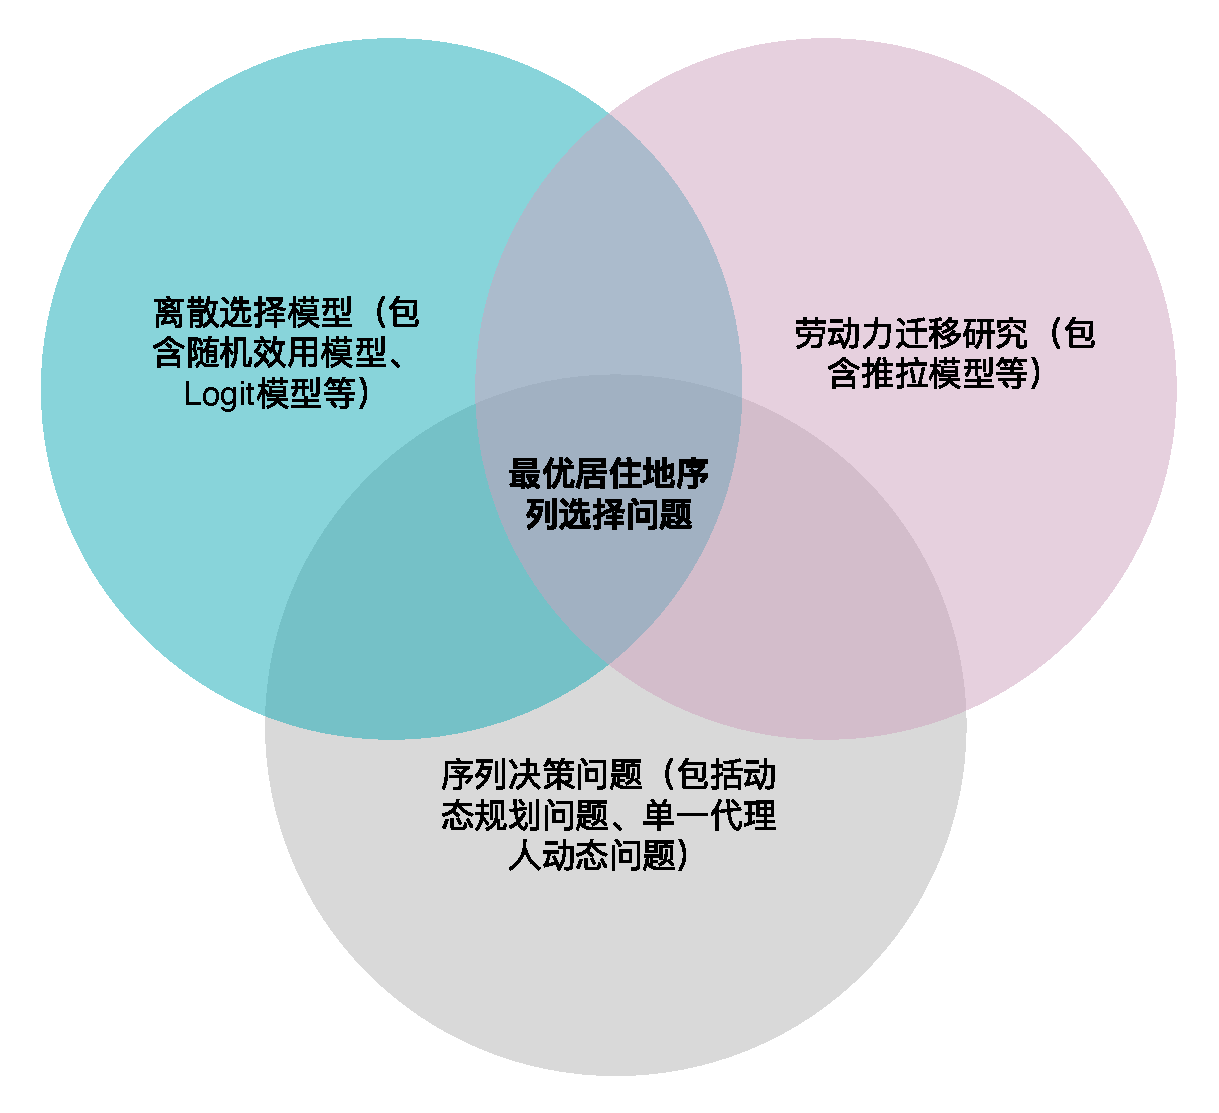
\includegraphics[width=0.65\textwidth]{images/optimal_residential_sequence.drawio.pdf}
\label{fig:最优居住地序列选择问题的理论来源venn diagram}
\end{figure}
























% ---------------------------------------- 理论模型 ----------------------------------------
\chapter{理论模型}

劳动力流动问题本质上极为复杂。经过前述分析,我们认识到,劳动力流动和迁移不应被简单地视为一次性经济活动,而应被理解为贯穿个体整个生命周期的持续决策过程。
假设决策者\footnote{文章中出现的个体指可以独立做出决策的经济单位,其形式可能为个人,也可能为家庭。为了消除歧义,后续将使用“决策者”一词替代。}有在多个地理位置之间自主选择的自由意志,每个位置均对应一种独特且互斥的收益流(payoff flow)。当决策者做出迁移决策后将承担相应的迁移成本。
这意味着劳动力流动的本质是一个“投资”决策。
决策者放弃当前的确定性(如本地工作),投资于一个充满不确定性但可能回报更高的未来(去大城市)。成本不仅是路费和短期收入损失,更是社会网络的断裂、制度性歧视(户籍)、以及巨大的心理压力。收益也不仅是更高的工资,更是子女的未来、更广阔的职业平台和个人价值的实现。
决策者在不同阶段根据自身状况和外部环境变化,不断权衡是否迁移、迁移到何处,以及迁移后如何实现自身利益最大化。


本文通过动态离散选择框架构建了一个迁移决策模型,用来分析人们在不同阶段如何做出迁移的选择,其必要性源于传统方法面临的三个关键问题。
第一,传统的静态模型无法反映人们在生命周期中因积累人力资本而导致的迁移意愿变化。简单来说,随着年龄、经验或技能的变化,人们对迁移的态度也会改变,而这些动态特征是静态模型无法捕捉的。  
第二,现实中每个人的情况都不同,比如风险偏好、处理信息的能力等。这些个人特质往往难以直接观测,但它们又会直接影响迁移决策,甚至与迁移行为相互作用。这种复杂的因果关系使得传统模型难以准确刻画实际情况。  
第三,不同地区之间的收益(如收入、生活质量等)并不是固定不变的,而是随着时间动态变化且存在长期关联。因此,我们需要一个能够考虑跨期影响的预期效用函数来更好地描述人们的决策过程。  
为此,本研究提出动态迁移决策模型(Dynamic Migration Decision Model, DMDM),以更贴近现实的方式分析迁移行为及其背后的逻辑。

\section{初步模型}

本文考虑一个封闭经济体,
人口流动仅发生在经济体内部,不存在国际移民或与外部世界的人口交换。
人口在各地区之间分布不均,并且随时间而动态变化。
假设人口的总量保持不变。
经济体由 $m$ 个离散地区组成,形成迁移网络$\mathcal{C} = \{1,2,\dots,m\}$,即个体决策者的居住地选择集。
各区域拥有固定的地理边界和空间关系,每个地区连通且可达,迁移连通性由$m$行$m$列的邻接矩阵$Adj=[j_{xy}\in\{0,1\}]$刻画。
不同的区域都具有独特的地区特征,这包括经济特征与非经济特征等,每个地区的特征会影响个体的迁移决策。
各地区的工资由本地劳动力市场决定。
时间被划分为离散的时期$t=\{0,1,2,\ldots,t,t+1,\ldots\}$。决策者获取效用,在每个时期以效用最大化为目标做出迁移决策。地区特征(如工资、就业机会)、经济状况和政策随时间变化,影响个体的预期和决策。

同时经济体中实施户籍制度。
令居民的出生地为其户口所在地$hukou$。
如果决策者的户口所在地与其当前所在不同,就会对其福利、基础设施的获取造成负面影响,从而降低效用的获取。反之,则会增加效用。户籍制度对于决策者的影响效果如图\ref{fig:户籍制度造成影响的途径}所示。
\footnote{
这样的经济体会产生迁移吗?
在劳动力自由流动的经济体中,地区间收入差异会因劳动力迁移而趋于收敛,但非经济因素的地区差异仍然存在。即使在非经济因素趋同的特殊情形下,由于决策者的地区偏好设定,劳动力流动仍将持续存在。此外,本文还引入了户籍制度障碍、家乡溢价和迁移成本,进一步制约了劳动力的自由流动,降低了地区收入差异收敛的能力。
}

\begin{figure}[!ht]
\centering
\caption{户籍制度造成影响的途径}
\label{fig:户籍制度造成影响的途径}
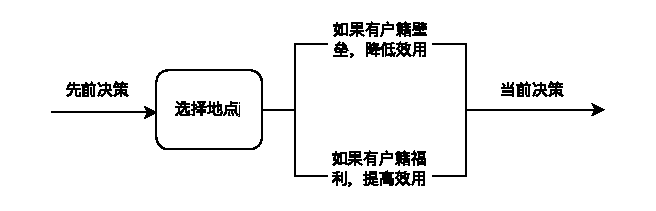
\includegraphics[width=0.8\textwidth]{images/户口影响.drawio.pdf}
\end{figure}


假设资产不影响居民的选择,考虑一个理性的决策者在$T$期生命周期内选择最优居住地序列。令$j_t \in \mathcal{C}$表示第$t$期的居住地选择,那么完整的选择序列可表示为$\mathcal{J}=\{j_1, j_2 ,\dots,j_T\}$。典型的居住地选择模式如表格\ref{tab:居住地选择序列可能的形式}所示。

\begin{table}[!ht]
\centering
\begin{tabular}{@{}ll@{}}
\hline
\multicolumn{1}{c}{\textbf{个体流动形式}} & \multicolumn{1}{c}{\textbf{居住地选择序列}}    \\ \midrule
\begin{tabular}[c]{@{}l@{}}\textbf{长期定居}:决策者在特定时间段内总是\\ 停留在同一个地区\end{tabular}                          & $\mathcal{J}=\{\dots, 1,1,1,1,1,\dots\}$ \\
\begin{tabular}[c]{@{}l@{}}\textbf{单向迁移}:如果 $j_p \neq j_q, \forall p\neq q$,那么\\ 个体就进行了迁移\end{tabular} & $\mathcal{J}=\{\dots, 1,2,3,4,5,\dots\}$ \\ 
\textbf{回流迁移}:返回到先前居住过的地区                      & $\mathcal{J}=\{\dots, 1,2,2,1,1,\dots\}$ \\ \bottomrule
\end{tabular}
\caption{居住地选择序列可能的形式}
\label{tab:居住地选择序列可能的形式}
\end{table}


决策问题由状态变量$x_t$刻画,其包含
个体特征(年龄、收入、家庭规模等)、
地区属性(房价、公共设施等)、
历史居住选择记录、
宏观经济环境
等因素。
状态转移服从马尔可夫过程,其转移概率为$p(x_{t+1}|x_t,j_t)$。

决策者在第$t$期从居住地$j$
\footnote{本文中$j$代表可选择的地点,而$j_t$代表个体在$t$期做出的具体选择。}
获得的地区效用为:
\begin{equation}
  \tilde{u}_t(j, x_t) = u_t(j, x_t)  +  \zeta_{jt}
  \label{eq:地区效用函数}
\end{equation}
其中$u_t(j, x_t)$为确定性效用项,
$\zeta_{jt}$为在任意时期和地点都独立同分布的随机扰动项,服从标准Gumbel分布$F(\zeta) = \exp(-\exp(-\zeta))$,且与状态变量$x_t$无关。


理性决策者做出选择的标准是选择使得效用最大化的选项:
\begin{equation}
  j_{it} = \arg\max_{j \in C} \{\tilde{u}_t(j, x_t)\}
\end{equation}

对于在选择集$\mathcal{C}$中选择$j$的概率可以写为:
\begin{equation}
\begin{split}
  Pr(\text{选择地点j})&=Pr(\tilde u_j > \tilde u_k, \forall k \neq j)
  \\&=Pr(u_j+\zeta_j>u_k+\zeta_k, \forall k \neq j)
  \\&=Pr(\zeta_k-\zeta_j<u_j-u_k, \forall k \neq j)
\end{split}
\label{eq:C中地点选择j的概率}
\end{equation}

在动态框架下,决策者具有前瞻性,并且通过最大化期望折现效用进行跨期优化。决策者在每期进行最优的居住地选择,或者说决策者选择$T$维的最优居住地选择序列$\mathcal{J}^*=\{j_1^*,j_2^*,\ldots,j_T^*\}$。每期的效用可以分为两部分,一是选择地点$j \in \mathcal{C}$带来的当期效用,二是折现的通过转移概率加权得到的未来期望效用。

假设折现因子为$\beta \in (0,1)$,决策者的目标是为从$t$期开始的期望折现效用最大值,这可以表示为:
\begin{equation}
  V_t(x_t, \zeta_{j_t}) = \max_{j_t \in \mathcal{C}} 
  \left\{ 
  \tilde{u}(j_t, x_t) + \beta \sum_{x_{t+1}} p(x_{t+1} | x_t, j_t) \cdot \mathbb{E}_{\zeta_{j_{t+1}}} [ V_{t+1}(x_{t+1}, \zeta_{j_{t+1}}) ]
  \right\}
\end{equation}
其中$\mathbb{E}_{\zeta_{j+1}} v_{t+1}(x_{t+1},\zeta_{j+1})$
为在状态 
$x_{t+1}$下,对所有可能随机扰动 
$\zeta$取期望后的长期效用。

那么决策者的基本问题就是在每个给定状态$x$和随机项 $\zeta_j$的情况下,选择最优居住序列$\mathcal{J}^*$使得全生命周期中的期望折现效用最大化,即:
\begin{equation}
  \max_{\mathcal{J}=\{j_1,j_2,\ldots,j_T\}} \mathbb{E} [ \sum_{t=1}^{T} \beta^{t-1} \tilde{u}_{j_t}(j_t,x_t) ]
\end{equation}

也可以使用迭代形式,即决策者每期都选择$j$来实现使得个体在生命周期中的总效用最大化,
令
$\begin{cases}
  v(j_{t},x_{t})=u(j_{t} ,x_{t})+\beta \sum_{x_{t+1}} p(x_{t+1}|j_t,x_t) \cdot \mathbb{E}_{\zeta_{j+1}} V_{t+1}(x_{t+1},\zeta_{j+1})
  \\
  \bar v(x_{t})=\mathbb{E}_{\zeta_{j_t}} v_{t}(x_{t},\zeta_{j})
\end{cases}$
,其中$E_{\zeta}$表示对 J 维向量$\zeta$的分布求期望\footnote{对于决策者而言收益冲击$\zeta$在做出居住地选择决策之前就已经实现,而$v(x,j)$ 和 $\bar v(x)$ 之间的区别在于,一个表示每个替代选择的延续值,而另一个表示在收益冲击实现之前所取的优化延续值的期望。},决策者基本问题的迭代形式为:
\begin{equation}
V(x,\zeta)=\max\limits_{j}[v(j,x)+\zeta_{j}]
\end{equation}

图片\ref{fig:migration_flow_resized2} 展示了一个动态规划决策过程。在离散周期$t$结束时或者下个周期$t+1$即将开始时,决策者根据在抽取到的随机收益冲击$\zeta$和状态转移概率$p(x_{t+1}|x_t,j_t)$双重不确定性的影响下通过Bellman方程做出决策,进入下一个周期$t+1$后获得该期的效用$\tilde u_{t+1}$。

\begin{figure}[!ht]
\centering
\caption{动态离散选择模型下的劳动力迁移决策流程图}
\label{fig:migration_flow_resized2}
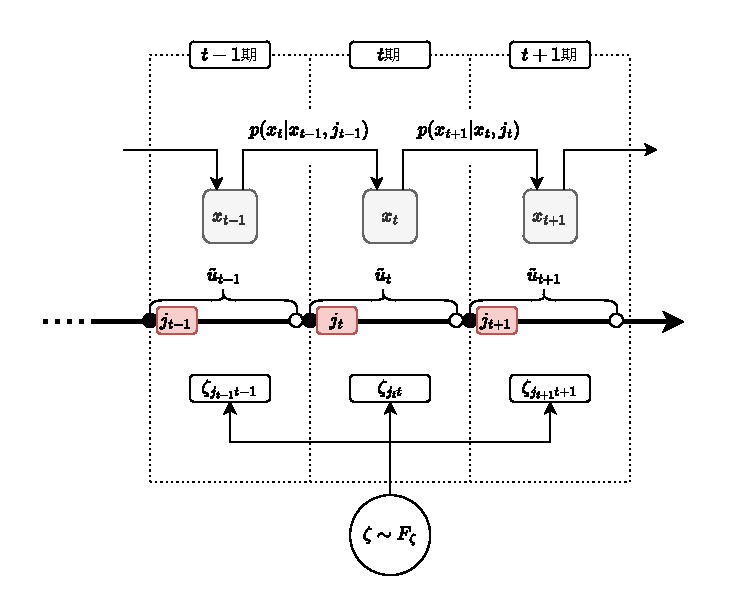
\includegraphics[width=0.9\textwidth]{images/dynamicsequence2.drawio.pdf}
\end{figure}

由于随机效用项$\zeta_j$独立同分布且服从 I 型极值分布,根据\textcite{mcfaddenConditionalLogitAnalysis1973,rustOptimalReplacementGMC1987,rustStructuralEstimationMarkov1994}的结论,可知:
\begin{equation}
  \exp(\bar v(x_t))=\sum\limits_{k=1}^{J}\exp(v(x_t,k_t))
\end{equation}
可知选择地点j的概率,即公式\ref{eq:C中地点选择j的概率},存在softmax函数形式,这是由Gumbel噪声的极值分布性质推导的:
\begin{align}
\rho(x,j)&=\exp(v(x,j)-\bar v(x))
\\&=\frac{\exp(v(x,j))}{\sum\limits_{k\in J} \exp(v(x,k))} \label{eq:地点选择概率}
\end{align}
这极大地优化了动态规划问题中期望值的计算,并且由于sotfmax函数输出的概率分布是平滑的,有利于策略迭代的稳定性。


%由于随机效用项$\zeta_j$独立同分布且服从 I 型极值分布,其概率累积分布为$F(\zeta_j)=\exp(-\exp(-\zeta_j+\bar \gamma))$,其中$\bar \gamma$为欧拉常数。

%$\max_j \left(v(x,j)+\zeta_j\right)$的期望为$\bar v(x) = E_\zeta V(x,\zeta)= \ln(\sum\limits_{k=1}^J \exp(v(x,k)))+\bar \gamma$。这表明$\exp(\bar v(x)-\bar \gamma)=\sum\limits_{k=1}^J \exp(v(x,k))$。将其简化为,$\exp(\bar v(x))=\sum\limits_{k=1}^J \exp(v(x,k))$。

%利用Gumbel分布的封闭性质,将选择地点$j$的概率事件表达式化为$\rho(x,j)=\exp(\bar \gamma + v(x,j) - \bar v(x))$,
%将$\bar v(x)$的定义式代入其中,化简后利用指数运算的特性可得动态离散选择中的地点选择概率\footnote{这实际上也是softmax函数的一种概率向量形式,可以在动态模型中通过$\bar v(x) = \ln (\sum \exp(v(x,k)))+\bar \gamma $将未来效用递归嵌入当前选择。}
%\begin{equation}
%  \rho(x,j)=\frac{\exp(v(x,j))}{\sum\limits_{k=1}^J \exp(v(x,k))}
%\end{equation}


\section{效用函数具体构成}

接下来为公式\ref{eq:地区效用函数}赋予具体形式,从而使其具有经济意义。
假设个体决策者$i \in \mathcal{N}$的
家乡为$h$,那么该点上可能的效用流为:
\begin{equation}
  \tilde u_{t}^h(j_t,x_t;\theta)=u_{t}^h(j_t,x_t;\theta) +\zeta_{j_t,t}
  \label{eq:家乡效用函数}
\end{equation}

假设收入的边际效用是固定的,居民可以在固定利率下自由借贷,那么居民的期望效用最大化问题就可以转化为预期永久收入\footnote{永久收入以现值形式记录。}
减去一次性付清的迁移成本。
\footnote{
假设效用函数的线性形式为$U(x)=a X$,其中a为边际效用参数。居民可在固定利率$r$下无限制借贷,预算约束满足消费现值等于收入现值。
居民可以留在原地(永久收入为$Y_h$)或迁移(永久收入为$Y_p$,后者需支付一次性迁移成本 $M$。
假设迁移成本 
$M$
为即期支出,且永久收入为永续年金。

若居民留在原地,其永久收入的现值为
$W_h = \sum\limits_{t=0}^\infty \frac{Y_h}{(1+r)^t}=\frac{Y_h}{r}$,
总效用为$U_h=a W_h = \frac{a Y_h}{r}$。
若居民选择迁移,需支付即期成本 
$M$
,迁移后的永久收入现值为
$W_h = \sum\limits_{t=0}^\infty \frac{Y_p}{(1+r)^t}=\frac{Y_p}{r}$,
由于迁移成本 
$M$
为即期支出,净现值为
$\mathcal{W}=W_p-M=\frac{Y_p}{r}-M$,
总效用为
$U_p=a(\frac{Y_p}{r}-M)$
迁移的条件为$U_p>U_h \Rightarrow a(\frac{Y_p}{r}-M) > a \frac{ Y_h}{r} \Rightarrow Y_p-Y_h > rM$。
期望效用最大化等价于选择净现值更高的选项,即$\max\{a(\frac{Y_p}{r}-M), a \frac{ Y_h}{r}\}$。
}
居民的基础效用由货币性收入、城市宜居度、家乡溢价减去迁移成本组成。令效用函数为如下形式:
\begin{equation}
  \begin{split}
    u_t^h(j_t,x_t;\theta)=&\alpha_0 \cdot w_{ijt}+\sum\limits_{s} \alpha_{s} \cdot y_{s}(j_t)  + \alpha_h \cdot I(j_t=h) 
    \\& + \alpha^p \cdot I(j_t \neq hukou) +\xi(j_t,\omega)-\kappa(j_t,j_{t-1},x_t)
  \end{split}
  \label{eq:家乡效用函数中的具体构成}
\end{equation}
其中$\theta$代表参数向量, $w(j_t,\omega_t)$为经济收益函数,衡量个体在当前位置通过劳动获得的经济收益,$\alpha_0$表示工资收入对效用的权重(边际效用);
$y_{s}(j_t)$为该居住地提供的非货币性舒适度(amenity)价值,如气候、公共服务、文化等,反映地理位置的非经济吸引力,$y_s$是第$s$种舒适度的量化指标(如教育质量指数),其边际效用由$\alpha_s$表示;
$\alpha_h \cdot I(j_t=h)$是对家乡的偏好溢价,$\alpha_h$衡量个体对出生地的情感依恋强度,其中$I(\cdot)$为指示性函数,当其中判断为真时返回1,否则为0,这意味着只有当当前所在地是家乡时效用才会额外增加$\alpha_h$;
$\alpha^p \cdot I(j_t = hukou)$为人户分离时的制度障碍效应,只有当所在地与户籍地不同时才会产生$\alpha^p$单位的效用增减;
$\xi(j_t,\omega)$为个体的地区偏好成分,
反映个体对某地点的长期偏好匹配(如文化契合度),仅当个体访问该地点时才能获知其具体值;
$-\kappa$为从其他区域前往地区$j$的迁移成本函数,负号表示迁移成本会降低效用,包括直接费用(如搬家费)和间接成本(如适应新环境的心理成本)。



公式\ref{eq:家乡效用函数中的具体构成}中,决策者的经济收益函数由多种因素组成。在不考虑时间因素的影响下,个体决策者$i \in \mathcal{N}$在地区$j \in \mathcal{C}$的收入设定为以下函数形式:
\begin{equation}
  w_{ij}=\mu_j + \nu_{ij} + G(X_i,a,t) + \eta_i + \varepsilon_{ij}(a)
  \label{eq:经济收益函数}
\end{equation}
地区基准收入$\mu_j$反映地区$j$的平均工资水平,
代表地区的经济基本面,如生活成本、区域产业聚集效应(如北京的传媒业、山西的采矿业)、政策红利(税收减免、人才补贴)等结构性特征,是所有在该地点个体的工资基准,
其与个体无关,仅取决于地点特征。
个体-地区匹配效应$\nu_{ij}$表征相同技能劳动者在不同地区的收入差异,
捕捉个体与地区的特殊适配性(如技能需求匹配、文化契合度),例如,程序员在科技中心可能获得更高的$\nu_{ij}$,
其具备匹配效应在个体驻留期间保持稳定,一旦个体进入地区 $j$,
$\nu_{ij}$固定不变,但迁移到新地区$k$ 时会生成新的 $\nu_{ik}$\footnote{在这点上与地区偏好$\xi$类似,但前者可通过工资和迁移选择共同推断,而后者仅能通过迁移选择推断。}。
匹配效应实现值$\nu_{ij} \sim F_\nu$在个体进入地区$j$后方可观测。
生命周期收入$G(X_i,a,t)$为线性函数,其包含三重要素,
个体特征$X_i$包含教育程度、性别等,
年龄效应$a$反映人力资本积累曲线,
时间趋势$t$捕捉技术进步等外生冲击。
量化系统性因素对工资的影响(如工作经验随年龄增长、宏观经济波动)。
$G$ 的影响在不同地区间相同(如教育回报无地区差异)。
个体固定效应$\eta_i$表征表示个体 $i$ 异质性中不随地区改变的固有能力或特质,
如先天能力、家庭背景等,无论迁移到哪里均保持恒定。
假设个体已知 $\eta_i$ 的值,并在决策中利用此信息。
暂时性随机效应$\varepsilon_{ij}(a)$代表短期波动或随机扰动项,服从i.i.d分布的当期扰动,
捕捉不可预测的工资波动(如临时绩效波动、经济冲击)。
假设$\varepsilon$服从期望为0的正态分布,并且独立于其他变量,随年龄和时间变化,个体无法预知其实现值\footnote{所以即使暂态效应对于每个地点都不同,但对居住地选择决策无持续影响。}。

如果发生了迁移($j_t \neq j_{t-1}$),同个决策者$i$的迁移成本$\kappa$设定为以下函数形式:
\begin{equation}
\begin{split}
  \kappa=I(j_t \neq j_{t-1}) \cdot [& 
  \gamma_{0 \tau}
  + \gamma_1 D(j_{t-1},j_t)
  - \gamma_2 I(j_t \in Adj(j_{t-1}))
  \\&
  - \gamma_3 I(j_t \in Pre)
  + \gamma_4 a
  -\gamma_5 n_j
  ]
\end{split}
\label{eq:迁移成本函数}
\end{equation}
$\gamma_{0\tau}$迁移中类型相关的的固定成本,随个体类型 $\tau$ 变化,从而捕捉未观测的异质性。例如:“定居型”个体(stayer type)的 $\gamma_{0\tau}$ 极高,几乎禁止迁移;“流动型”个体的 $\gamma_{0\tau}$ 较低,更易迁移。不同类型的群体分布由对应的概率$\pi_\tau$给出,并且满足$\sum\limits_{\tau}^{} \pi_\tau=1$。
$\gamma_1 D(\ell^0, j)$为迁移距离效应,是 $D(\ell^0, j)$ 的线性成本(以大圆距离衡量),距离越远,成本越高($\gamma_1 > 0$)。  
$-\gamma_2 \chi(j \in A(\ell^0))$是相邻地区效应,若目标地点 $j$ 与当前地点 $\ell^0$ 相邻(即 $j \in A(\ell^0)$),则成本减少 $\gamma_2$。
相邻地区迁移可能因文化相似、信息透明或交通便利而成本更低($\gamma_2 > 0$)。  
$-\gamma_3 \chi(j = \ell^{-1})$为历史地区效应(回流效应),
其定义为若目标地点 $j$ 是个体曾居住过的历史地点 $\ell^{-1}$,则成本减少 $\gamma_3$。
这是因为返回熟悉地区可能因现存社会网络或无需重新适应而成本更低($\gamma_3 > 0$)。  
$+\gamma_4 a$代表年龄障碍效应,表明迁移成本随年龄 $a$ 线性增加,年龄越大,迁移的心理或生理成本越高($\gamma_4 > 0$)。  
$-\gamma_5 n_j$为目标地区规模成本效应,
目标地区人口规模 $n_j$ 越大,迁移成本减少 $\gamma_5 n_j$。  
这是因为
大规模地区可能有更多潜在支持(如亲友网络、服务机构),减少安家难度,从而降低迁移成本($\gamma_5 > 0$),符合“引力模型”中人口规模吸引迁移的经典结论。  
$I(j_t \neq j_{t-1})$为迁移指示函数 ,仅当目标地点 $j \neq \ell^0$ 时,迁移成本生效(否则为0)。  这确保个体留在原地时无需支付迁移成本。

迁移成本中参数的经济含义如表格\ref{tab:迁移成本参数释义}所展示。
\begin{table}[!ht]
  \centering
  \caption{迁移成本参数释义}
  \label{tab:迁移成本参数释义}
  \begin{tabularx}{\textwidth}{@{}llX@{}}
    \toprule
    \multicolumn{1}{c}{\textbf{参数符号}} & \multicolumn{1}{c}{\textbf{参数含义}} & \multicolumn{1}{c}{\textbf{参数意义}} \\ \midrule
    \multicolumn{1}{c}{$\gamma_{0\tau}$} & 类型异质效应 & 捕捉不同类型的异质性,可以解释为何有些人从不迁移,识别“定居型”人群可针对性地设计激励措施(如搬迁补贴)。\\ 
    \multicolumn{1}{c}{$\gamma_1$} & 物理迁移成本 & 个体与其携带物必然因为物理法则而产生运输成本。 \\ 
    \multicolumn{1}{c}{$\gamma_2$} & 相邻地区效应 & 反映地理邻近性的普遍优势。 \\ 
    \multicolumn{1}{c}{$\gamma_3$} & 历史地区效应 & 返回历史地区因熟悉度获得折扣,体现路径依赖。 \\ 
    \multicolumn{1}{c}{$\gamma_4$} & 年龄障碍效应 & 针对不同年龄群体制定差异化迁移政策(如青年人才引进计划)。\\ 
    \multicolumn{1}{c}{$\gamma_5$} & 规模成本效应 & 大地区吸引力不仅体现在经济机会(如工资 $\mu_j$),也直接降低迁移成本。\\ \bottomrule
  \end{tabularx}
\end{table}


此外,由于暂态效应$\varepsilon$服从期望为0、标准差差为\(\varepsilon_{it}\)的正态分布,已知经济收益函数设定为公式\ref{eq:经济收益函数}。
令$\phi$表示标准正态分布的概率密度函数,处于地点$j$的个体$i$在时期$t$的经济收益函数的密度函数$\Psi_{it}$为:
\begin{equation}
  \Psi_{it}=\phi(\frac{w_{it} - \mu_{jt} - G_{it} - \nu_{ijt} - \eta_i }{\sigma_{\varepsilon_{it}}})
  \label{eq:经济收益似然贡献}
\end{equation}
这是决策者的似然贡献之一。

\section{状态转移概率}

本文将决策者在不同时期的迁移决策组成一个序列,并将其建模成一个马尔可夫决策过程(Markov Decision Process, MDP)。
MDP包括两个核心假设,即决策具有目标性和Markov性。决策的目标性是指决策者在每个状态下选择一个行动,其究极目标是最大化某种累积奖励,也就是他的长期收益。
状态转移的 Markov 性 指下一时刻的状态仅依赖于当前状态和采取的行动,而与过去的状态和行动无关
\footnote{在许多实际场景中,个体的迁移决策确实主要基于当前的状态(如当前所在城市的生活成本、就业机会、家庭因素等),而不是过去的迁移历史。因此,本文的Markov 性假设是合理的。}。
状态变量转移概率描述的是在选择了特定位置$j_{t}$的情况下,从状态 $x_t$ 移动到新状态 $x_{t+1}$的条件可能性。
本文假设状态变量转移概率具有马尔可夫性
,即系统的未来状态仅依赖于当前状态和当前决策,与过去的历史无关,这意味着:
\begin{equation}
  p(x_{t+1}|x_{t},j_{t},x_{t-1},j_{t-1},\ldots)=p(x_{t+1}|x_{t},j_{t})
\end{equation}
该假设,符合沉没成本理论,大大简化了问题的复杂度。

根据先前的模型假设,决策者只有在迁移到某个地点时才能了解真实的工资和效用匹配值,因此新的目的地是随机抽取新的匹配值的。
具体而言,本文将其设置为:
\begin{equation}
  p(x_{t+1}|x_t,j_t)=
  \begin{cases}
    % 迁移
    \frac{1}{m^\omega}
    , &\text{发生迁移从而产生随机抽取}
    \\
    % 不迁移
    1
    , &\text{没有迁移}
    \\
    % 其他
    0
    , &\text{其他情况}
  \end{cases}
\end{equation}


将状态变量 \( x \) 分解,实际为包含一个 \( M \) 维的最近位置向量 \( \ell \)、一个 \( m \) 维的与位置相关的工资和效用信息向量 \( \omega \),以及个人年龄 \( a \)。为了计算简便,状态向量定义为 \( x = (\tilde{x}, a) \),其中 \( \tilde{x} = (l^0, l^1, x_0^0, x_0^1, x_\xi^0, x_\xi^1) \)。其中,\( l^0 \) 表示当前位置 \( j_t \),\( l^1 \) 表示上一个位置 \( j_{t-1} \)。索引 \( x_0^0 \) 和 \( x_0^1 \) 分别对应于当前和先前位置的工资匹配值 (\( v_{i l^0} \), \( v_{i l^1} \)),而 \( x_\xi^0 \) 和 \( x_\xi^1 \) 则表示效用匹配值 (\( \xi_{l^0} \), \( \xi_{l^1} \))。年龄 \( a \) 捕捉了个体状态的时间维度。

1. 无迁移 (\( j_{t+1} = j_t \)):如果个体停留在当前位置 (\( j_{t+1} = l^0 \)),状态分量保持不变 (\( \tilde{x}' = \tilde{x} \)),年龄增加 1 (\( a' = a + 1 \))。转移概率为 1,反映工资和效用匹配 (\( v_{i l^0} \), \( \xi_{l^0} \)) 保持不变。

2. 返回先前位置 (\( j_{t+1} = j_{t-1} \)):当个体返回先前位置 (\( j_{t+1} = l^1 \)) 时,当前位置和先前位置互换 (\( l'^0 = l^1 \), \( l'^1 = l^0 \))。工资和效用匹配指数会相应更新:先前位置的工资指数变为当前工资指数 (\( x_0'^0 = x_0^1 \)),当前位置的工资指数变为先前工资指数 (\( x_0'^1 = x_0^0 \))。同样,效用指数也会互换 (\( x_\xi'^0 = x_\xi^1 \), \( x_\xi'^1 = x_\xi^0 \))。年龄递增 (\( a' = a + 1 \)),转移概率为 1。这保留了历史匹配信息,反映了路径依赖性,而无需重新抽取。

3. 迁移到新位置 (\( j_{t+1} \notin \{ j_t, j_{t-1} \} \)):如果个体移动到新位置 (\( j_{t+1} = j \)),则当前位置更新 (\( l'^0 = j \)),并且先前位置变为之前的当前位置 (\( l'^1 = l^0 \))。新的工资和效用匹配分别从具有 \( n_0 \) 和 \( n_\xi \) 个可能值的离散分布中随机抽取,索引分别为 \( s_0 \in \{1, \dots, n_0\} \) 和 \( s_\xi \in \{1, \dots, n_\xi\} \)。因此,\( x_0'^0 = s_0 \) 和 \( x_\xi'^0 = s_\xi \),同时保留先前位置的匹配 (\( x_0'^1 = x_0^0 \)、\( x_\xi'^1 = x_\xi^0 \))。年龄递增 (\( a' = a + 1 \)),转移概率为 \( \frac{1}{n^2} \)(假设 \( n_0 = n_\xi = n \)),反映了对新地点匹配的独立且均匀的抽取。

4. 无效转移:上述情况未涵盖的任何转移的概率为 0,以确保仅考虑有效的地点选择。

并且,该设置通过索引匹配值而不是存储其显式值,从而压缩状态空间,以利于求解数值。
转移概率反映了决策者对新地点的探索,其中工资和效用信息仅在抵达时才会显示,而历史数据则会保留以备潜在的返回迁移。这种结构支持在信息不完整的情况下进行动态决策,平衡对新位置的探索和对已知路径相关信息的依赖。

\section{劳动力迁移决策}

由于地区偏好效应和个体固定效应仅与个体特征相关,而且暂态效应仅在迁移行为发生后随机产生,因此这些因素无法影响迁移决策。
在不同地区$j$和$k$之间,仅有地区平均工资$\mu$、地区匹配效应$\nu$和非经济因素存在地区间差异。
地区选择通过影响收入水平而产生作用,劳动力将倾向于选择具有更优劳动力市场条件、更高地区匹配效应和更高宜居度条件的目的地。
然而,这种选择必须同时满足预期收益需超过户籍制度障碍、迁移成本、心理成本(如恋家效应)以及随机效用冲击等因素造成的阻力。
简言之,外部条件对决策者效用的提升必须足以克服迁移过程中的各类障碍,这恰如公式\ref{eq:迁移motivation}所示。
\begin{equation}
\begin{split}
  Pr(\text{选择k})&= Pr(u_k - u_j > \zeta_j - \zeta_k) 
  \\&= Pr(
  \text{地区k的客观因素} - \text{地区j的客观因素} 
  > 
  \underbrace{\alpha^p}_{\text{制度}} + \underbrace{\alpha^h}_{\text{心理}} + \underbrace{\kappa}_{\text{迁移成本}} + \underbrace{
  \zeta_j - \zeta_k}_{\text{外生冲击}} 
  )
  \\&= p >0
\end{split}
\label{eq:迁移motivation}
\end{equation}

至此,模型刻画出了在有限生命周期内,决策者每期面临制约与摩擦,在迁移网络$\mathcal{C}$中自由选择最优住址$j_t$,从而最大化自身的长远利益。这些不同时期的选择构建出了最优居住地选择序列$\mathcal{J}$。这意味着迁移可以是多次的,可撤回的。同时,这也可以刻画出了劳动力迁移的自由性,与现实世界中的行为是融洽的。




% ---------------------------------------- 实证部分 ----------------------------------------
\chapter{实证处理}

\section{模型上} 

采取动态规划方法的一个缺陷在于计算上很容易陷入维度的诅咒(curse of dimensionality)。出于实证处理的简便处理,本文将对于模型中一些难以计算的点进行简便假设。

\subsection{年龄效应}
出于简化,
本文参照以往的计量经济学经验,
将年龄效应\(G\)设置为年龄的有待估参数的一次项和二次项的和。即,将\ref{eq:家乡效用函数中的具体构成}中的$G$设置为:
$$G=r_1 a + r_2 a^2$$


\subsection{非参数离散混合方法} 

基于上述模型设定,公式\ref{eq:家乡效用函数中的具体构成}中的地区偏好$\xi$、公式\ref{eq:经济收益函数}中的个体固定效应$\eta$、地区匹配效应$\nu$以及暂态效应$\varepsilon$的具体函数形式仍未确定。若无法解决这一识别问题,将难以准确计算决策者的效用函数和期望值。因此,有必要对这些随机项的概率分布施加合理的假设和约束条件。

出于计算上的简便,
本文使用支撑点离散化方法。
对于任何不知道其分布的 $F$,我们可以找到最佳近似分布 $\hat F$ 来近似。对于连续分布的变量$F$,离散的 $\hat F$ 是一组有限的支撑点组成,每个支撑点都有对应的概率值,即$\{(x_i, p_i)\}, 1 \leqslant i \leqslant N$ 的组合,其中 $x_i$ 是离散点,$p_i$ 是其概率,$N$ 为给定的支持点数。
对于每个$q_r, (1\leqslant r \leqslant n )$,计算对应的效用值,用这些有限的效用值来代替连续效用的积分。
通过该处理后,模型变为有限状态的动态规划问题,可以直接构建似然函数并进行最大似然估计。
相较于蒙特卡洛模拟,该方法可以避免随机噪声,适合精确的极大似然估计。

由于假设分布围绕 0 对称,因此仅需要 $\frac{M-1}{2}$ 个支持点即可进行估计。

令 $p_i = \frac{1}{N}, \forall i$。

对于$\nu$
在每个地点中个体都有从地区匹配效应的分布中抽取一个值,假设这个分布是一个有限集合上的均匀分布,$Y=\{\nu(1),\nu(2)...\nu(n_{\nu})\}$
其结果是$\omega^{i}_{\nu}$,$\omega^{i}_{\nu}(j)$代表在地点j的匹配效应,$1\leqslant j\leqslant N_i$,$N_i$是$i$到达过的地方的数量
总共有$\{\omega^{i}_{\nu}(1),\omega^{i}_{\nu}(2)...\omega^{i}_{\nu}(j)...\omega^{i}_{\nu}(N_i)\}$

$\xi$
地区匹配偏好也是如此
来自于$\Xi=\{\xi(1),\xi(2)...\xi(n_{\xi})\}$
其结果是$\omega^{i}_{\xi}$

$\eta$ 表示每个个体工资的固定成分(例如长期能力或个体特质)。
假设其分布是一个对称的离散分布,具有7个支持点。每个支持点有相等的权重。
因为是离散分布,只需要估计 3个参数:分布的中间点(中心趋势)和离散范围。
固定效应代表长期的工资差异来源,例如教育水平、经验等。
选择离散分布是为了简化复杂的连续分布,同时通过支持点捕捉关键的分布特性(如中心趋势和差异性)。
$\eta$的离散分布提供了一种对长期工资特质的简化建模方式,减少计算复杂度,同时保留重要信息。
固定效应也是如此
来自于$H=\{\eta(1),\eta(2)...\eta(n_\eta)\}$
其结果是$\omega^{i}_{\eta}$

暂态效应$\varepsilon$在本质上是一种外生冲击,所以可以假设为服从期望为$0$的正态分布$N(0,\sigma^2)$,
保留了异方差特质以变容纳更多的异质性。
数学上$\varepsilon$表示工资的短期波动成分,比如由于经济周期、随机冲击等导致的变化
假设$\varepsilon_{it}$(某人在某个时间的短期波动)来源于一个均值为零的正态分布,其方差$\sigma_{\epsilon}$随人而异
对于每个人,$\sigma_\varepsilon(i)$来自一个离散分布(4 个支持点,均匀分布),因此需要估计 4 个参数
$\varepsilon$反映工资中不可预测的临时变化,例如经济不确定性或工作绩效波动
允许$\sigma_\varepsilon(i)$因人而异捕捉到工资短期波动的个体差异性(例如高风险行业可能有更大波动)
在建模中,$\varepsilon$允许方差随个体变化,体现了个体的异质性,这进一步增加模型的灵活性,使其能够更好地拟合数据。

暂态效应来自于一个期望为$0$的正态分布,但是假设其异方差使其可以可以容纳更多的异质性。
即$\varsigma=\{\sigma_{\epsilon}(1),\sigma_{\epsilon}(2)...\sigma_{\epsilon}(n_{\epsilon})\}$,
其结果是$\omega^{i}_{\epsilon}$。

表格\ref{tab:未观测到的变量表}总结了以上未知分布变量的设定。

\begin{table}[!ht]
\centering
\caption{未观测到的变量表}
\label{tab:未观测到的变量表}
\begin{tabular}{@{}ccccc@{}}
\toprule
变量 & 变量符号 & 分布假设 & 数量 & 抽取结果 \\ \midrule
地区匹配效应 & $\nu$ & $Y=\{\nu(1),\nu(2)\ldots\nu(n_{\nu})\}$ & n & $\omega^{i}_{\nu}(j)$\\
地区偏好 & $\xi$ & $\Xi=\{\xi(1),\xi(2)\ldots\xi(n_{\xi})\}$ & 1 & $\omega^{i}_{\xi}$ \\
固定效应 & $\eta$ & $H=\{\eta(1),\eta(2)\ldots\eta(n_\eta)\}$ & 1 & $\omega^{i}_{\eta}$ \\
暂态效应的方差 & $\varepsilon$ & $\varsigma=\{\sigma_{\varepsilon}(1),\sigma_{\varepsilon}(2)\ldots\sigma_{\varepsilon}(n_{\varepsilon})\}$ & 1 & $\omega^{i}_{\varepsilon}$ \\ \bottomrule
\end{tabular}
\end{table}


参数向量的可能实现组成一个集合,用$\Omega(N_{i})$表示,未观测到的因素组成一个$m_{i}+3$维的参数向量$\omega^{i}=(\omega^{i}_{\xi},\omega^{i}_{\eta},\omega^{i}_{\epsilon},\omega^{i}_{\nu}(1),\omega^{i}_{\nu}(2)...\omega^{i}_{\nu}(N_{i}))\in \Omega$。


对于公式\ref{eq:迁移成本函数}迁移成本函数中的异质性成本$\gamma_{0\tau}$,
模型假设随个体类型 $\tau$ 变化,从而捕捉未观测的异质性。
具体而言,本文将其分为分为3种类型。
类型1:高迁移倾向,低迁移成本,高不确定性容忍度。
类型2:中等迁移倾向,中等迁移成本,中等不确定性容忍度。
类型3:低迁移倾向,高迁移成本,低不确定性容忍度。
“定居型”个体(stayer type)的 $\gamma_{0\tau}$ 极高,几乎禁止迁移;
“流动型”个体的 $\gamma_{0\tau}$ 较低,更易迁移。
个体i属于类型k的概率为$\pi_k$,并且满足$\sum\limits_{k}^{} \pi_k = 1$。
每种类型的比例$\pi_1, \pi_2, \pi_3$作为模型参数被估计。
类型k的个体的效用函数为$u_{ijt}^k$,
模型可表示为:
$$V_{ijt}^k = u_{ijt}^k + \varepsilon_{ijt}^k + \beta^k E_t[V_{t+1}^k|d_{ijt}=1]$$
其中$k\in{1,2,3}$表示类型。


\section{似然函数}

由上文可知个体存在两种似然概率函数贡献,即公式\ref{eq:地点选择概率}和公式\ref{eq:经济收益似然贡献}。
通过个体在其历史轨迹中给出的两种似然贡献,
我们得到了类型为$\tau$的个体$i$的似然函数

即在所有可能的不可观测变量的组合下,个体在所有时期中的观测收入$w_{it}$上选择地点的概率$\rho_{it}$的乘积:
\begin{equation}
  L_{i}(\theta_{\tau})=\frac{1}{n_{\nu}n_{\epsilon}n_{\xi}(n_{\nu})^{N_{i}}} \sum\limits_{\omega^{i}\in\Omega(N_{i})}(\prod\limits_{i=1}^{T_{i}} \psi_{it}\lambda_{it})
\end{equation}

由于模型允许存在异质性

让$L_{i}(\theta_{\tau})$代表tau类型个体的似然函数,其中$\theta$是该个体的待估参数向量

样本的似然函数是一个混合类型的联合对数似然函数,把每个观测i的贡献相加
\begin{equation}
\Lambda(\theta)=\sum\limits_{i=1}^{N}\log(\sum\limits_{\tau=1}^{K}\pi_{\tau}L_{i}(\theta_{\tau})) 
\end{equation}
其中混合比例由$\pi_{\tau}$给出,且$\sum\limits_{\tau=1}^{K}\pi_{\tau}=1$
每个个体i都做出了贡献
这是在给定参数$\theta_{\tau}$的条件下,个体$i$在类型$\tau$下的似然。即,个体i可能属于某种类型,似然函数
$L_i(\theta_{\tau})$捕捉了该个体数据与类型$\tau$相关的匹配度。
混合似然$\sum_{\tau=1}^{K} \pi_{\tau} L_i(\theta_{\tau})$这表示对所有类型的加权平均,权重是$\pi_{\tau}$,即每种类型的概率。通过这种加权求和,模型允许每个个体属于不同的类型,并通过类型的权重(概率)来加权它们的贡献。

每个个体可能属于不同的类型,这些类型有不同的收入和行为模式。每个数据点i来自某个成分,但成分的归属是未知的,因此需要将每个数据点的似然表示为各成分似然的加权和,然后取对数并求和得到整个样本的对数似然。因此通过混合模型,能够捕捉到个体之间的异质性。


如此,通过最大似然计算,就可以得到各种参数的似然估计。

\section{迁移成本的似然函数}

已知先前推倒中


% subsection 实证模型 (end)

\section{数据上}

地区数据的界限
由于劳动力的迁移在不同省之间呈现趋势 但在迁入大省中仍然存在人口净流出市 这说明劳动力移动的法律边界和现实边界存在重合 但是最好应该以市为标准 当然这一准则不包括某些政策带来的效应
上面说了为什么界限要往下卡在市,下面说一下为什么界限不继续往下到区或者村。首先是政策往往以市为最小执行单位;其次是在市内迁移中个人会为了出于固定资产投资等非模型考量的原因,这些原因并不是因为在迁居的地区能提供更好的个人预期工资
市级包含了县、乡、村等行政级别 每个市都包含了城市与农村(虽然城市化率略有不同)避免了城乡之间的划分对立


人口数据的界限
许召元2007

在我国存在广泛的农民工进城现象 大多数农民工只是暂时居住在


本研究使用CFPS2010年至2022年年两期数据构成面板进行影响评估。CFPS采用的是内隐分层、多阶段、多层次、与人口规模成比例的概率抽样方式,样本覆盖除中国港澳台、新疆、西藏、青海、内蒙古、宁夏和海南之外的其他省/市/自治区。这些地区的人口占全国的95\%左右,因此,CFPS的数据是一个具有全国代表性的高质量数据库。

关键结果变量为个人的年总收入 (PIncome)。本研究选取的关于个人总收入的变量为“qk601”(2010年) 和“pincome”(2014 年) 。在面板数据中,两个变量统一命名为“PIncome”。该变量来自 CFPS 问卷的 “K 部分: 个人收入”,具体题目为“您 ( 去年)个人的年总收入是元?”。CFPS在公布历期数据之前,对收入部分结果进行了修正,以满足各年之间的可比性。控制变量。参考以往研究 (卜茂亮等,2011; 黄国英、谢宇,2017; 谭燕芝等, 2017; 周广肃、孙浦阳,2017) 并结合CFPS数据的可获得性和完整性,本文选取的控制变量包括地域 (所在省份)、常住地 (城镇或农村)、性别、民族、年龄、受教育年限、婚姻状态、自评健康状况、认知能力、非认知能力、对自己未来的自信心和职业等。其中CFPS的非认知能力来自访员在理解能力、配合程度、接人待物水平、回答的可信程度和语言表达能力5个方面对受访者的评价平均得分; 认知能力包括语文和数学方面的测试得分 (黄国英、谢宇,2017)

本文选取2010年至2022年都存在记录的个体,

个体决策者的微观数据来源于自CFPS从2010年到2022年间的数据,
其记录了个人的迁移轨迹(将访问当年的地址视作居住地址)、年龄、收入等。


本文使用的地理数据包含我国31个省份(由于现行制度的不同和数据收集的难度,本文的数据排除了香港特别行政区、澳门特别行政区以及台湾省地区),
其中常住人口数量、人均可支配收入、自然灾害数据、城市人口数据、医疗数据、教育数据等数据来自于国家统计局公布的数据统计年鉴。


对于宜居度,本文将以下数据设为宜居度指标:

气候数据:
由于气候和空气质量在短期内发生变化的可能性较小,气候的对比不是局部发生变化的,以及气候数据在劳动力迁移决策中是用于进行横向对比而非纵向对比的,所以本文选用常量对每个省份的空气质量、日照时间、平均气温进行跨时间同一数值赋值。

气象:

本文的气象数据来自visualcrossing,通过获取每个城市每日的天气数据,将其从原先的日级别(day level)和城市级别(city level)的数据汇总成年级别(year level)与省级别(province level)的格式。具体操作请见于本文github代码库的代码。

最高温度平均数 最低温度平均数 紫外线强度 体感舒适天数  空气质量优良率


宜居度包括:
自然禀赋:
生活水资源


房价收入比:
本文参考\textcite{LiHuiFangJieFangJieShouRuBiYuLiuDongRenKouChangQiJuLiuYiYuanLaiZiLiuDongRenKouDeWeiGuanZhengJu2019}选取房价收入比作为房价的宜居度表现形式。
房价数据来自于xxx。com网站

商业资源:
本文还使用各省每万人连锁餐饮门店数与每万人社会零售消费品总额(亿元)代表商业资源


本文的公共服务包含以下:

1.地方教育:
地方教育经费、地方医疗经费来自各省地方财政局网站公布的数据。
由于教育的变量存在高度相关性
所以使用主成分分析法将教育变量整合为一个指标

2.地方医疗:
同样的
对于医疗资源使用熵值法合成一个指标

3.市政设施:
城市用水普及率
城市燃气普及率
每万人拥有公共交通车数量
人均公园绿地面积(平方米/人)
每万人拥有公共厕所(座)
使用PCA主成分生成一个指标


对于省份的地理指标,本文将其进行如下处理:

距离数据各省市以其省会为,经纬度源自geopy的Nominatim,计算方法则基于其geodesic方法。
该方法基于WGS84椭球模型,考虑地球的扁率使得精度更高,使用Vincenty算法迭代计算两点间的最短测地线距离。
\footnote{
具体而言,
已知地球的
长半轴为$a = 6378137.0$ 米(WGS-84椭球的赤道半径),
扁率为$f = 1 / 298.257223563$,
则短半轴为$b = a(1 - f)$。
给定两点以弧度表示的经纬度坐标 $ P_1(\phi_1, \lambda_1) $ 和 $ P_2(\phi_2, \lambda_2) $,
计算经度差$\Delta\lambda = \lambda_2 - \lambda_1$,
再利用使用 Vincenty 公式求解两点之间的中心角 $\sigma$。
测地线距离 $d$ 的最终公式为$d = b \cdot A \cdot \sigma$,
其中$A$是与椭球扁率相关的修正系数。
}

在研究省份之间的迁移成本或区域经济联系时,地理邻接性是一个重要的影响因素。邻接省份通常具有更紧密的经济、文化和交通联系,这些因素会显著影响人口流动、资源配置以及区域协同发展。
邻接省份可能在区域性政策上更具一致性,这降低了迁移者的制度适应成本;邻接省份之间可能存在更紧密的经济联系,例如产业链上下游关系,为迁移者提供更多就业机会。
因此,为了量化省份之间的邻接关系,本文根据我国省级行政区划的地图信息,构建了一个邻接矩阵 A。
设 A 是一个 $N \times N$的方阵(其中 $N$ 为省份数量),每行和每列分别对应一个省份。对于矩阵中的任意元素 $a_{m,n}$而言,其对应的数值代表$m$省与$n$省之间的邻接关系,若邻接则取$1$,否则为$0$。
在构建邻接矩阵时,本文假设省份之间的邻接关系仅由地理边界决定,而不考虑其他因素(如交通网络密度或行政合作程度)。此外,受数据限制,本文暂不考虑海峡等自然障碍对邻接关系的影响。同样的,本文排除了港澳台三个地区。

中华人民共和国教育部发布的《中国语言文字概况(2021)》指出,我国有56个民族,是一个多民族、多语言、多方言、多文字的国家。普通话和规范汉字是国家通用语言文字,是中华民族通用的语言文字。
现代汉语有标准语和方言之分。
汉语方言通常分为十大方言:官话方言、晋方言、吴方言、闽方言、客家方言、粤方言、湘方言、赣方言、徽方言、平话土话。各方言区内又分布着若干次方言和许多种“土语”。其中使用人数最多的官话方言可分为东北官话、北京官话、冀鲁官话、胶辽官话、中原官话、兰银官话、江淮官话、西南官话八种次方言。
以往文献中速来有讨论方言对于劳动力流动的影响,
例如\textcite{HuangZongYeFangYanDuiShengJiRenKouQianYiDeYingXiang2020,LiQinFangYanPuTongHuaYuZhongGuoLaoDongLiQuYuLiuDong2014}等,但是这些文献中往往将方言的影响局限于语言是否相同。
本文基于比较语言学中对于我国方言的大量研究,提出采用
基于树形结构的最近公共祖先(LCA)距离来划分各省市之间的方言亲近度。
\footnote{
对于一个有根树形结构$T=(V,E)$,其中
$V$表示树的顶点集合;
$E\subseteq V \times V$表示边的集合;
任意其中两个节点$u$和$v$,它们的最近公共祖先 $LCA(u,v) $定义为
$LCA(u,v)=\arg \max_{w\in V} depth(w)$,
其中 $w$ 是同时满足是 $u$ 和 $v$ 的祖先;$w$ 在树中的深度最大。
换句话说,$LCA(u,v)$ 是从根节点到 $u$ 和 $v$ 的路径上的最后一个公共节点。
}
公式\ref{eq:方言相似度}展示了对于各省代表性语言计算亲近度的方式。
\begin{equation}
  \label{eq:方言相似度}
  \text{方言相似度}=\frac{1}{1+\text{LCA depth}}
\end{equation}
本文使用的语言谱系树如图\ref{fig:linguistic_tree}所示。
\begin{figure}[!ht]
\centering
\caption{语言谱系树}
\label{fig:linguistic_tree}
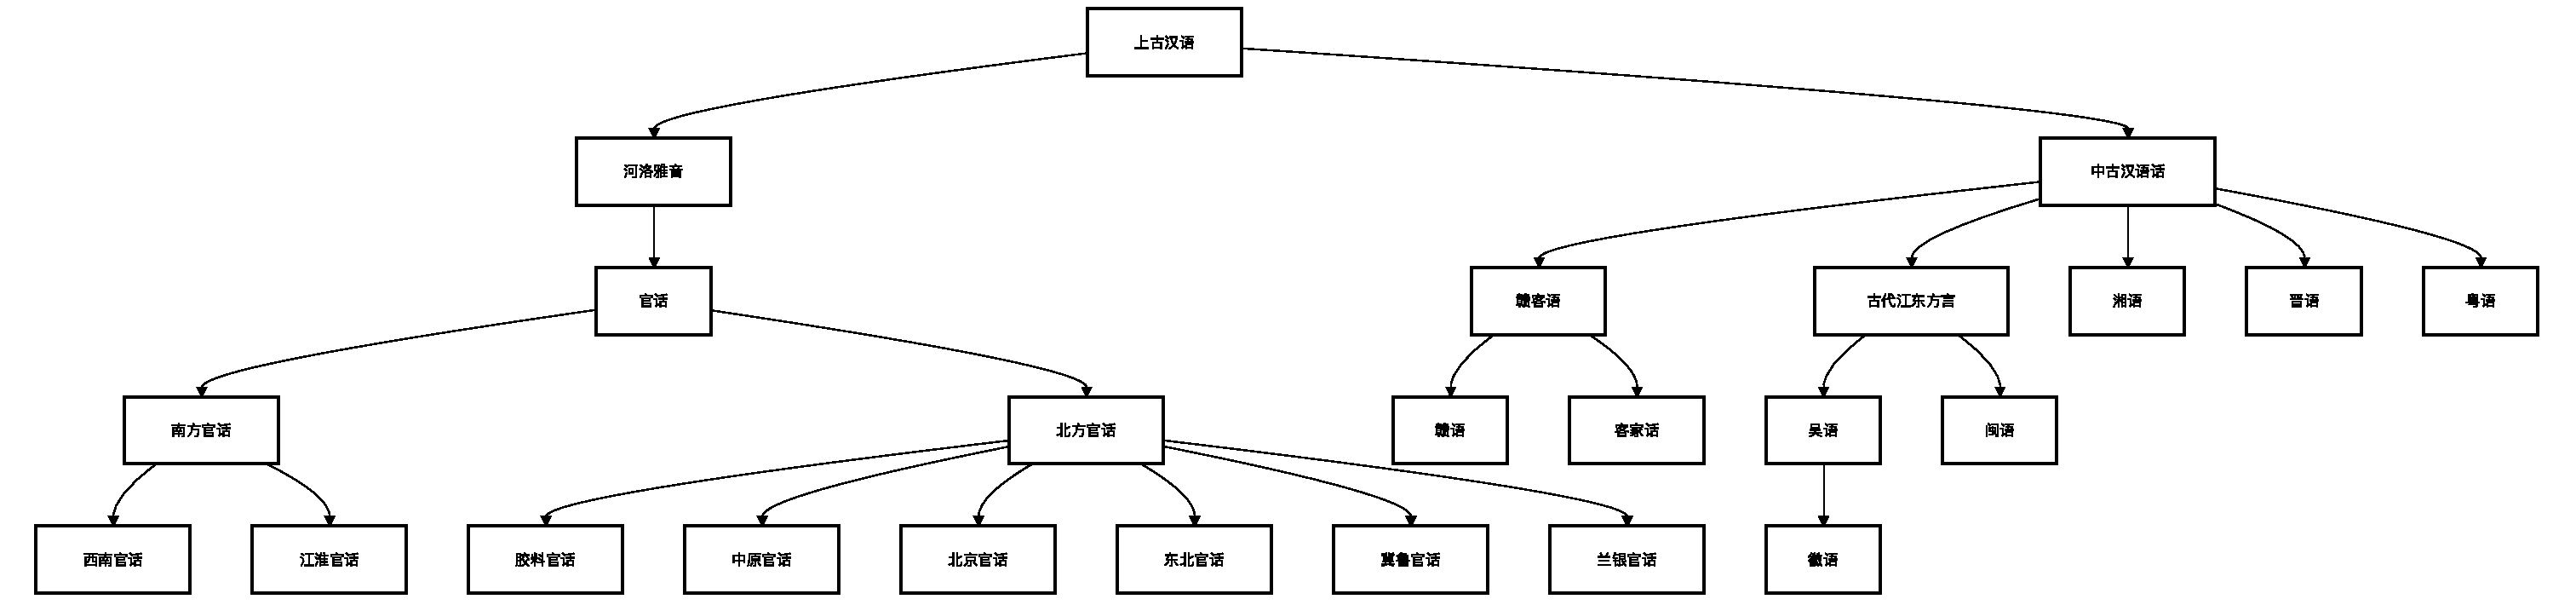
\includegraphics[width=\textwidth]{images/linguisitc_tree.drawio.pdf}
\end{figure}
由于各省之间存在大量的方言,并且现实中缺乏各方言在各省市中的人口分布数据,本文根据《中国语言地图集》选取各省的代表性语言作为其方言指标。值得注意的是部分省份由于内部存在大量完全分割的语言,例如江苏就包括吴语与江淮官话,本文选取流入人口较多的苏州、无锡一带的吴语作为其代表性语言;又例如山东省内部存在胶辽官话、冀鲁官话、中原官话,本文以济南市的冀鲁官话作为其代表性语言。本文的具体设置如表格\ref{tab:方言分布表}所示。
同时本文还将各省市的普通话普及率纳入模型,数据来源则参考了\textcite{YuWeiQiGuoMinPuTongHuaNengLiDeJiBenZhuangKuangYuFaZhanTaiShi2018},从CGSS中获取。




\begin{table}[!ht]
\centering
\caption{方言分布表}
\begin{tabularx}{\textwidth}{@{}ccXccX@{}}
\toprule
\textbf{代表性方言} & \textbf{数量} & \multicolumn{1}{c}{\textbf{省份}} & \textbf{代表性方言} &\textbf{数量}  & \multicolumn{1}{c}{\textbf{省份}}\\
\midrule
西南官话 & 6 & 湖北省、广西壮族自治区、重庆市、四川省、贵州省、云南省 &晋语 & 2 &山西省、内蒙古自治区\\
东北官话 & 3 &辽宁省、吉林省、黑龙江省 & 北京官话  &1 &北京市\\
吴语 & 3 &浙江省、上海市、江苏省& 赣语  &1 &江西省\\
中原官话 & 3 &河南省、陕西省、青海省 &胶辽官话  &1& 山东省\\
冀鲁官话 & 2 &天津市、河北省、山东省 &湘语  &1 &湖南省\\
闽语 & 2 &福建省、海南省 &粤语  &1& 广东省\\
兰银官话 & 2 &甘肃省、宁夏回族自治区 &其他  &2& 西藏自治区、新疆维吾尔自治区\\
\bottomrule
\end{tabularx}
\label{tab:方言分布表}
\end{table}


本文对于复合指标的获取如表格所示

\section{方法上} % (fold)
\label{sub:方法上}

基于以上的推导,
在代码中需要先求出个体的似然,
而个体的总似然是迁移选择概率和工资观测概率的乘积,
那么集体的似然函数同时对未观测的随机效应(固定效应、地区匹配效应等)进行积分(离散求和):
\begin{equation}
  L_{i}=\sum\limits_{\text{所有随机效应组合}}[\prod_{t}\rho(x_{t},j_{t})\cdot P(w_{t}|\text{随机效应}) ]
\end{equation}

本文采用混合似然估计法(Mixed Likelihood Estimation)进行动态离散选择模型的参数求取。由于模型涉及高维状态空间与跨期动态关联性,计算过程具有三重复杂性:其一,个体选择行为需通过贝尔曼方程递归求解;其二,状态转移矩阵需处理多重内生性关联;其三,价值函数收敛需满足跨期一致性条件。

传统计量工具(如Stata)受限于矩阵运算效率与迭代算法架构,在应对此类包含200+状态变量、需进行10\^6量级矩阵运算的复杂场景时,存在计算耗时指数级增长与内存溢出的双重瓶颈。
为此,本文构建基于Python的数值计算框架,与传统的Stata相比,Python在实现复杂的动态离散选择模型方面具有显著优势:
首先,Python的开源生态系统提供了丰富的科学计算库,如\lstinline{NumPy}、\lstinline{Pandas}和\lstinline{PyTorch},这些库为处理大规模面板数据和实现复杂的优化算法提供了强大支持。特别是\lstinline{PyTorch}的自动微分功能,使得计算复杂模型的梯度变得简单高效,这在传统Stata环境中难以实现。
其次,Python的面向对象编程范式使得模型的各个组件可以被清晰地封装,提高了代码的可读性和可维护性。在本项目中,我们将模型的不同部分(如个体似然函数\lstinline{IndividualLikelihood}、参数估计器\lstinline{ModelEstimator}等)封装为独立的类,使得整体架构更加清晰。
此外,\lstinline{joblib}库提供的并行计算能力显著提高了计算效率,特别是在处理大量个体似然函数计算时;
本文设计逆向归纳算法(Backward Induction),通过倒序年龄迭代(从T期至$t_0$期)动态求解各状态节点的期望价值函数(EV矩阵),确保跨期决策路径的全局最优;
并运用SciPy优化器进行参数空间搜索,通过蒙特卡洛模拟生成选择概率曲面,最终实现模型参数在95\%置信区间内的有效估计。


对于求取参数的方法,传统上使用Newton线搜索方法上求解似然函数最大值,虽然收敛速度快,但计算海塞矩阵需要消耗大量资源。
虽然可以通过对似然函数进行LU分解,在计算海塞矩阵的逆时提供可靠帮助,降低数值不稳定性,
但计算海森矩阵的代价仍然较高,尤其是在参数较多时。
本文做出改进,
采取以自动微分(\lstinline{PyTorch})为核心,使用现代优化算法Quasi-Newton方法中的L-BFGS方法避免收敛困难和数值不稳定,并利用离散化与并行处理提升效率。
BFGS是一种拟牛顿法,通过迭代逼近目标函数的海塞矩阵的逆矩阵,从而避免直接计算二阶导数。它只需要利用梯度信息来更新海森矩阵的近似,使得每次迭代都能更准确地找到下降方向。在高维参数空间中,避免了直接计算海森矩阵的高计算成本。
在具体的梯度计算中,自动微分通过计算图追踪运算过程,利用链式法则自动计算导数,避免数值微分的截断误差。当模型复杂、参数众多,且需要频繁计算梯度时(如神经网络训练),自动微分显著优于手动编码梯度。对于需要高阶导数或大规模并行计算的情况尤为适合。
具体而言,
本文使用类方法分装待估参数
类继承
\lstinline{torch.nn.Module},所有参数为\lstinline{torch.nn.Parameter},支持自动梯度计算。

本文对于固定效应和地区匹配效应upsilon等支撑点离散化方法的处理与原作者的做法保持一致,
通过网格遍历求和。
对于已经用支撑点离散近似后的参数,在进行网格搜索时,
\lstinline{joblib.Parallel}支持将数据存储在磁盘上的内存映射文件中,这样多个进程可以共享同一份数据,
而无需每个进程都复制一份,从而显著降低内存消耗并提升 I/O 效率。

本文的优化方法基于深度学习,
模型估计结果对初始值存在一定敏感性,
初始值的选择可能会影响收敛速度和结果。例如,如果真实值接近-0.1,好的初始值能加快收敛。
虽然L-BFGS优化器在一定程度上缓解了这一问题,但仍需根据经济学理论进行初始值赋予能促进优化方法的应用,例如距离增加可能降低迁移概率,因此\lstinline{gamma_distance}的预期应该为负,将其初始值设为负符合理论预期,有助于引导优化方向。


本文中一些变量如表格\ref{tab:_实证与程序中的变量定义}所示。

\begin{table}
\centering
\caption{实证与程序中的变量定义}
\begin{tabularx}{\textwidth}{@{}ccXX@{}}
\toprule
变量符号 & 代码符号 & 含义 & 数据来源\\
\midrule
$\alpha_0$ & alpha0 & 经济性收入截距 &\\
$\alpha_1$ & alpha1 & 对于房价收入比作为宜居度的边际效用&\\
$\alpha_H$ & alphaH & 恋家溢价&\\
$\alpha_P$ & alphaP & 户籍制度惩罚&\\
$r_1$ & r1 & 年龄效应一次性系数& \\
$r_2$ & r2 & 年龄效应二次性系数& \\
 & houseprice & &\\
\bottomrule
\end{tabularx}
\label{tab:_实证与程序中的变量定义}
\end{table}

% ---------------------------------------- 估计结果 ----------------------------------------
\chapter{估计结果}

本文尝试回答一下几个问题:
\begin{itemize}
  \item 影响劳动力流动的因素是什么?到底哪些因素是负面因素(迁移摩擦)?
  \item 不同人群是否面对不同的劳动力迁移摩擦阻力?
  \item 本地的福利待遇对于迁移是否显著?这意味着是否可以通过政府补贴购买人才
  \item 
\end{itemize}


\textcite{XiaYiRanChengShiJianDeMengMuSanQianGongGongFuWuYingXiangLaoDongLiLiuXiangDeJingYanYanJiu2015} 利用 2005 年 1\%人口抽样调查中劳动力流动的微观数据与 220 个地级市的城市特征 数据研究发现公共服务对劳动力流入产 生 吸 引 力,同 时 房 价 对 劳 动 力 流 入 也 有 正 向 作 用,他 们 认 为这是因为房价“资本化”了部分未观察到的公共服务或城市特征,此文关注点不在房价,而且使 用的普查 数 据 没 有 覆 盖 近 十 年 来 中 国 房 价 暴 涨 的 阶 段。

\section{基准回归与子样本分析} % (fold)


标准回归下得到的估计系数如下表格\ref{tab:基准回归系数}所示。
\begin{table}[!ht]
\centering
\caption{基准回归系数}
\begin{tabularx}{\textwidth}{@{}cXXX@{}}
\toprule
\midrule
\bottomrule
\end{tabularx}
\label{tab:基准回归系数}
\end{table}



McFadden’s Pseudo R²:用于快速评估模型解释力和向非技术受众展示结果。


农村劳动力回流存在吗?农村户口更容易回流吗?


\section{拟合优度} 

预测准确性 (Prediction Accuracy) 
要求模型能够准确地预测每个个体的选择行为或结果。
更关注局部性能(即单个样本的预测)。
可能对噪声敏感,尤其是在样本量较小或数据质量较差的情况下。

模拟校准 (Simulated Calibration) 
要求模型能够捕捉系统的整体动态特性,即使它无法完美预测单个样本的行为。
更关注全局性能(即整体数据的统计特性)。
对噪声相对不敏感,因为模拟校准关注的是长期趋势和分布特性。

\textbf{预测准确率(Prediction Accuracy)}

根据模型的预测结果与实际观测值进行比较,计算预测准确率或其他分类指标。

适用性:通过比较模型预测的选择概率与实际选择结果,计算正确预测的比例。直接评估模型的预测性能,尤其适用于分类问题。

常用指标:

- 准确率 (Accuracy): 预测正确的比例。

- 精确率 (Precision)、召回率 (Recall) 和 F1 分数。

- ROC 曲线下的面积 (AUC)。

优点:直观,特别适合评估模型在实际劳动力状态(如是否回流)预测中的表现。

缺点:可能过于简化,无法捕捉概率分布的细微差异,且对类别不平衡的数据敏感。

建议:在劳动力回流问题中,预测准确率可以作为辅助指标,特别是在政策分析中需要评估模型对回流决策的预测能力时。结合混淆矩阵(Confusion Matrix)可以进一步分析模型在不同状态(如回流 vs. 非回流)上的表现。


\textbf{模拟校准 (Simulated Calibration)}

定义 : 使用估计的模型参数生成模拟数据,并将模拟数据的统计特性(如均值、方差等)与实际数据进行比较。

用途 : 验证模型是否能够重现数据的关键特征。

局限性 : 需要额外的模拟步骤,计算成本较高。

\textbf{敏感性分析}


\section{异质性人群的回归} 

其中关于经济性收入的参数,其估计结果如下表格\ref{tab:经济性参数的回归系数}所示。
\begin{table}[!ht]
\centering
\caption{经济性参数的回归系数}
\begin{tabularx}{\textwidth}{@{}cXXX@{}}
\toprule
\midrule
\bottomrule
\end{tabularx}
\label{tab:经济性参数的回归系数}
\end{table}


\section{从回归结果看待迁移摩擦}


\begin{table}[!ht]
\centering
\caption{迁移摩擦}
\begin{tabularx}{\textwidth}{@{}cXXX@{}}
\toprule
\midrule
\bottomrule
\end{tabularx}
\label{tab:迁移摩擦}
\end{table}



\section{迁移成本的具体构成}






% ---------------------------------------- 结论 ----------------------------------------
\chapter{结论与展望}

当然以城乡二元对立为代表的思想在我国依旧有非常重要的应用 因为我国依旧有大量依附于城乡关系的社会体系、福利体系等种种重要的制度
甚至在研究二元对立话题中依旧可以引入例如Rosen Roback这样的经典模型
例如 
\textcite{GuoDongMeiChengXiangRongHeDeShouRuHeFuLiXiaoYingYanJiuJiYuYaoSuPeiZhiDeShiJiao2023}指出城乡融合的收入和福利效应研究——基于要素配置的视角
但对于在破除劳动力迁移摩擦、开放劳动力要素自由流动的当下
抛开这种二元对立的思想是越来越重要的
这也自然而然地引出了空间均衡与最有选址两种思路



由于普遍偏好事少离家近的特征,政策可以针对性地对周边省份进行补贴
相反 对于十分遥远地区的人力资源 即使补贴了显性的迁移成本 也存在较长的文化、心里距离 所以在边际上可能并不值得投入



本文可以改进的地方:

添加约束

添加宏观变量

使模型作为微观基础从而宏观化
\textit{近年来,一些研究将上述两种基础模型结合起来,在空间均衡模型中加入了微观层面的动态迁移决策特征。这些动态一般均衡迁移模型明确考虑了空间工资差异的来源及其对净迁移和总迁移的影响,并允许存在不同类型的空间障碍,如劳动力重新配置摩擦和信息摩擦。这类模型特别关注迁移如何作为调节各地劳动力市场长期均衡的机制。例如,Coen-Pirani(2010)开发了一个动态一般均衡模型,强调了个体迁移决策中的不可观测异质性。该模型刻画了总迁移流动和净迁移流动的共同模式,其中前者由个体匹配的偶然冲击驱动,后者由持续的生产率冲击驱动。工人会迁移到正受到生产率冲击的地区,并在迁移后发现其偶然匹配的质量。新迁移的工人比长期居住者更可能继续迁移,因为后者选择留在某地是由于他们已经获得了相对较好的匹配。该校准模型可以解释为何人口流入较多的地区往往也伴随着较多的流出,这一现象在仅研究净流入的模型中无法得到解释。结合偶然匹配效应的空间均衡模型还能够解释新迁入工人与迁出工人在年龄、教育和行业等方面的相似性,这些特征无法仅通过个体位置选择模型或仅基于可观测工人异质性或地点特定冲击的模型来解释。}

从而引入其他变量

以家庭为基本单位


% ---------------------------------------- 附录 ----------------------------------------
\newpage
\appendix

\chapter{McFadden条件概率}

个体选择选项j的条件是其总效用最大,即
$u_j + \zeta_j > u_k + \zeta_k, \forall k \neq j$。
这可以转化为
$\zeta_j - \zeta_k > u_k - u_j, \forall k \neq j$。
假设误差项$\zeta_j$独立且服从相同的极值分布,则对于每个$k \neq j$,有
$\Pr(\zeta_j > \zeta_k + (u_k - u_j)) = \frac{1}{1 + \exp(u_k - u_j)}$。
在RUM模型中,当误差项独立时,选择j的概率为所有选项k的独立事件同时发生的概率,即
$P_j = \prod\limits_{k \neq j} \Pr(\zeta_j > \zeta_k + (u_k - u_j))$。
代入单个事件的概率表达式,选择j的概率是所有$k \neq j$的条件概率的乘积
$P_j = \prod\limits_{k \neq j} \frac{1}{1 + \exp(u_k - u_j)}$。
对$P_j$取对数
$\ln P_j = - \sum_{k \neq j} \ln(1 + \exp(u_k - u_j))$。
通过指数函数的性质,将上述表达式转换为
$P_j = \frac{\exp(u_j)}{\sum\limits_{k \in C} \exp(u_k)}$。

\chapter{效用等价于收入的特殊情况}
假设效用函数的线性形式为$U(x)=a X$,其中a为边际效用参数。居民可在固定利率$r$下无限制借贷,预算约束满足消费现值等于收入现值。
居民可以留在原地(永久收入为$Y_h$)或迁移(永久收入为$Y_p$,后者需支付一次性迁移成本 $M$。
假设迁移成本 
$M$
为即期支出,且永久收入为永续年金。

若居民留在原地,其永久收入的现值为
$W_h = \sum\limits_{t=0}^\infty \frac{Y_h}{(1+r)^t}=\frac{Y_h}{r}$,
总效用为$U_h=a W_h = \frac{a Y_h}{r}$。
若居民选择迁移,需支付即期成本 
$M$
,迁移后的永久收入现值为
$W_h = \sum\limits_{t=0}^\infty \frac{Y_p}{(1+r)^t}=\frac{Y_p}{r}$,
由于迁移成本 
$M$
为即期支出,净现值为
$\mathcal{W}=W_p-M=\frac{Y_p}{r}-M$,
总效用为
$U_p=a(\frac{Y_p}{r}-M)$
迁移的条件为$U_p>U_h \Rightarrow a(\frac{Y_p}{r}-M) > a \frac{ Y_h}{r} \Rightarrow Y_p-Y_h > rM$。
期望效用最大化等价于选择净现值更高的选项,即$\max{a(\frac{Y_p}{r}-M), a \frac{ Y_h}{r}}$。

\chapter{Rust极值分布}
公式中的随机效用项假设服从于一类极值分布
We assume that $\zeta_j$ is drawn from the Type I extreme value distribution. In this case, using arguments due to McFadden (1973) and Rust (1987), we have
$$\exp\left(\bar{v}(x)\right) = \sum_{k=1}^J \exp\left(v(x, k)\right)$$

这表示如果变量服从一类极值分布,那么$\exp\left(\bar{v}(x)\right)$可以表示为所有$v(x, k)$的指数和
它意味着,在状态x 下,选择某一选项j的概率与效用的指数值成比例。
这个性质广泛用于预测个体选择的分布。

\chapter{地点选择概率}
$\rho(x,j)=\frac{\exp(v(x,j))}{\sum\limits_{k=1}^{J} exp(x,k)}$

Probability that a person in state $x$ will choose location $j$ can then be written as
$$\rho(x,j)=\exp[v(x,j)-\bar v(x)]$$
% section 附录_证明 (end)证明

\chapter{log} % (fold)

令$\mathcal{K}_{it}=(\mathcal{K}_{it}^{0},\mathcal{K}_{it}^{1})$表示当前位置和上一个位置

已知\ref{eq:地点选择概率},
个体i在t时期选择目的地的似然概率是$\lambda_{it}(\omega^{i},\theta_{\tau})$
同时在
\begin{equation}
  \lambda_{it}(\omega^{i},\theta_{\tau})=\rho(x,j)=\rho_{h(i)}(\ell(i,t),\omega_{\nu}^{i}(\mathcal{K}_{it}^{0}),\omega_{\nu}^{i}(\mathcal{K}_{it}^{1}),\omega_{\xi}^{i}(\mathcal{K}_{it}^{0}),\omega_{\xi}^{i}(\mathcal{K}_{it}^{0}),a_{it},\ell^{0}(i,t+1),\theta_{\tau})
\end{equation}
公式表明个体的选择不仅受到过去历史(如上一个地点和上一个选择)和随机效应(如匹配效应和暂态效应)的影响,还考虑了个体的长期偏好和未来选择的影响。
通过对这个似然函数进行建模,我们可以估计个体在特定情况下做出选择的概率,从而理解个体在复杂环境下如何做出决策。


由于暂态效应服从期望为$0$的正态分布,并且已知经济收益函数设定为公式\ref{eq:经济收益函数},
令$\Psi$表示标准正态分布的概率累积函数,$\phi$表示标准正态分布的概率密度函数,可知经济收益函数的密度函数为
\begin{equation}
  \Psi_{it}(\omega^{i},\theta)=\phi(\frac{w_{it} - \mu_{\ell^{0}(i,t)}-G(X_{i},a_{it},\theta)-\nu(\omega_{nu}^{i}(\mathcal{K}_{it}^{0}))-\eta(\omega_{\eta}^{i})  }{\sigma_{\epsilon}(\omega_{\epsilon}^{i})})
\end{equation}
其中$\mu_{\ell^{0}(i,t)}$:是个体i在位置$\ell$基础工资水平;$G(X_i, a_{it}, \theta)$:代表个体$i$在时间$t$受到的外部影响(如经济环境、工作特征等);$\nu(\omega_{\nu}^i(\mathcal{K}_{it}^0))$、$\eta(\omega_{\eta}^i)$:分别是地区匹配效应和固定效应,它们是收入的随机组成部分,影响个体的收入;$\sigma_{\epsilon}(\omega_{\epsilon}^i)$:表示暂态效应的标准差,它反映了短期收入波动的程度。

这是在时期$t$给定个体$i$的选择和随机效应(如匹配效应、固定效应等),观察到收入$w_{it}$的概率概率,即被观测收入的似然概率。


\chapter{a}


To specification, factors including but not limited to as follow:

- income improvement. Higher income by comparison induces migration. 

- house price. Most researches agree the effect coulde be U-shaped.

- public service is a very large genre, we try to avoid such big word. It is a combination of all kinds of government-provided goods and natural resources. And the richer diveristy and better quality local government can provide, more migration is induced.

- weather

- hazzards

- cultural barrier is another big word genre, including but not limited to language barrier, habits, identity recognition and 

- direct migration cost, a total amount of present money paid for the transfer from one place to another. 迁移成本模型: 迁移成本模型考虑了个体在选择居住地时需要支付的成本(如搬家费用、适应新环境的成本等)。在考虑这些成本的情况下,个体可能会选择效用次优的居住地以避免高迁移成本。


\newpage
%\bibliography{Papers}
%\bibliographystyle{gbt7714-plain}
%\bibliographystyle{gbt7714-author-year}
\printbibliography[heading=bibliography,title=参考文献]
\end{document}
